\documentclass[bwprint]{gmcmthesis}
% \documentclass[withoutpreface,bwprint]{gmcmthesis}

\usepackage{pdfpages}
\usepackage{subcaption}
\usepackage{fancyvrb}
\usepackage[backend=biber,style=gb7714-2015]{biblatex}

\addbibresource{references.bib}
\graphicspath{{figures/}{image/}}
\numberwithin{figure}{section}
\renewcommand{\thefigure}{\arabic{section}-\arabic{figure}}
\newcommand{\figref}[1]{图~\ref{#1}}
\newcommand{\tabref}[1]{表~\ref{#1}}
\emergencystretch=3em

\title{ESG 报告数据智能提取与分析：证据约束型长文档结构化抽取模型}
\baominghao{No.00000001}
\schoolname{上海工程技术大学}
\membera{杨哲}
\memberb{邱宇强}
\memberc{王恒岳}

\begin{document}
\maketitle

\begin{abstract}
上市公司 ESG 报告通常以长 PDF 形式披露，具有页数多、表格与正文混排、指标口径差异大、定量与定性信息并存等特点。本文将赛题中的 ESG 指标识别任务抽象为 report-indicator 证据约束型结构化抽取问题：给定报告集合 $D$ 与指标集合 $Q$，对每一对 $(d_i,q_j)$ 先在解析后的内容块空间中召回候选证据，再由大语言模型在候选证据范围内输出固定 JSON 结构，并保留 evidence\_quote、page\_no 与 block\_id 以支持复核。

本文使用 200 份 A 股、北交所及港股上市公司 ESG 类 PDF 报告，构建 65 个覆盖 E、S、G 三个维度的指标，其中定量指标 35 个、机制性布尔指标 15 个、定性描述指标 15 个。MinerU 解析结果形成 10528 页、17740555 个 Markdown 字符和 235662 个内容块。全量构造 13000 个 report-indicator 任务，运行结果中 found 为 7777 条、missing 为 5223 条、error 为 0 条；该分布用于描述结构化抽取输出状态，不作为人工标注评价结论。进一步地，本文设计后处理与质量诊断规则，识别 value/unit 缺失、比例误作数量、金额误作数量、零事件归一、证据过短和标题式机制证据等风险，并通过 Streamlit 复核系统将结果查看、证据定位、风险样本与 CSV 下载串联为可追溯闭环。

\keywords{ESG 报告\quad 长文档抽取\quad 证据约束\quad 候选证据召回\quad 结构化信息抽取\quad 质量诊断}
\end{abstract}

\tableofcontents
\newpage

\section{问题重述}
\subsection{ESG 报告结构化抽取任务}
赛题要求围绕上市公司 ESG 报告完成数据采集、预处理、指标体系构建、定量与定性指标识别、结构化输出和结果展示。ESG 报告披露实践受到 GRI、ISSB 和 TCFD 等框架影响\parencite{gri2021,issb2023,tcfd2017}，但企业实际报告不同于单一表格数据源，其披露内容分散在正文、表格、章节标题、指标索引和附录中，同一指标在不同公司之间也常使用不同名称、单位和叙述方式。因此，本文不把任务处理为整篇文档问答，而是建模为可定位证据驱动的结构化抽取问题。

\subsection{定量、定性与机制性指标差异}
定量指标要求识别数值及单位，例如温室气体排放总量、能源消耗总量、员工培训小时数等；定性指标要求保留语义完整的原文片段，例如 ESG 战略、绿色产品与服务、员工权益保障等；机制性布尔指标关注报告是否披露制度、措施或治理安排，例如反腐败机制、ESG 治理架构和碳排放管理措施。三类指标的证据形态不同，决定了后续候选召回、字段约束和风险规则不能采用同一模板。

\subsection{研究目标与边界}
本文研究目标是从公开 ESG PDF 报告中形成可追溯的结构化结果，而非对企业 ESG 表现进行评分、排名或投资判断。输出字段保留 evidence\_quote、page\_no、block\_id 和 risk\_tag，使评审者可以从结构化数据回到报告证据。模型评价侧重运行结果分布、字段完整性、风险样本和复核闭环；在缺少完整人工真值集的前提下，不把自动运行状态解释为人工标注层面的评价指标。

\newpage
\section{数据集与文档特征分析}
\subsection{报告来源与样本构成}
本文采集并整理 200 份上市公司 ESG 类 PDF 报告。报告标识中可可靠提取证券代码、公司简称、年份和报告类型，由此得到 200 个唯一证券代码和 198 个公司简称。样本中 2025 年报告 196 份，2026 年报告 4 份；代码形态上，A 股或北交所代码 182 份，港股代码 18 份；报告类型包括 ESG 报告 171 份、可持续发展报告 18 份、ESG 暨社会责任报告 11 份。现有元数据未提供可靠行业字段，因此本文不作行业分布扩展解释。

\begin{table}[htbp]
\centering
\caption{数据集与解析规模摘要}
\label{tab:dataset-summary}
\begin{tabular}{ll}
\toprule
项目 & 数值 \\
\midrule
原始 PDF & 200 \\
公司数（文件名） & 198 \\
唯一证券代码 & 200 \\
解析成功报告 & 200 \\
解析总页数 & 10528 \\
Markdown 总字符数 & 17740555 \\
表格标记总数 & 6713 \\
图片引用总数 & 30465 \\
\bottomrule
\end{tabular}

\end{table}

\begin{figure}[htbp]
\centering
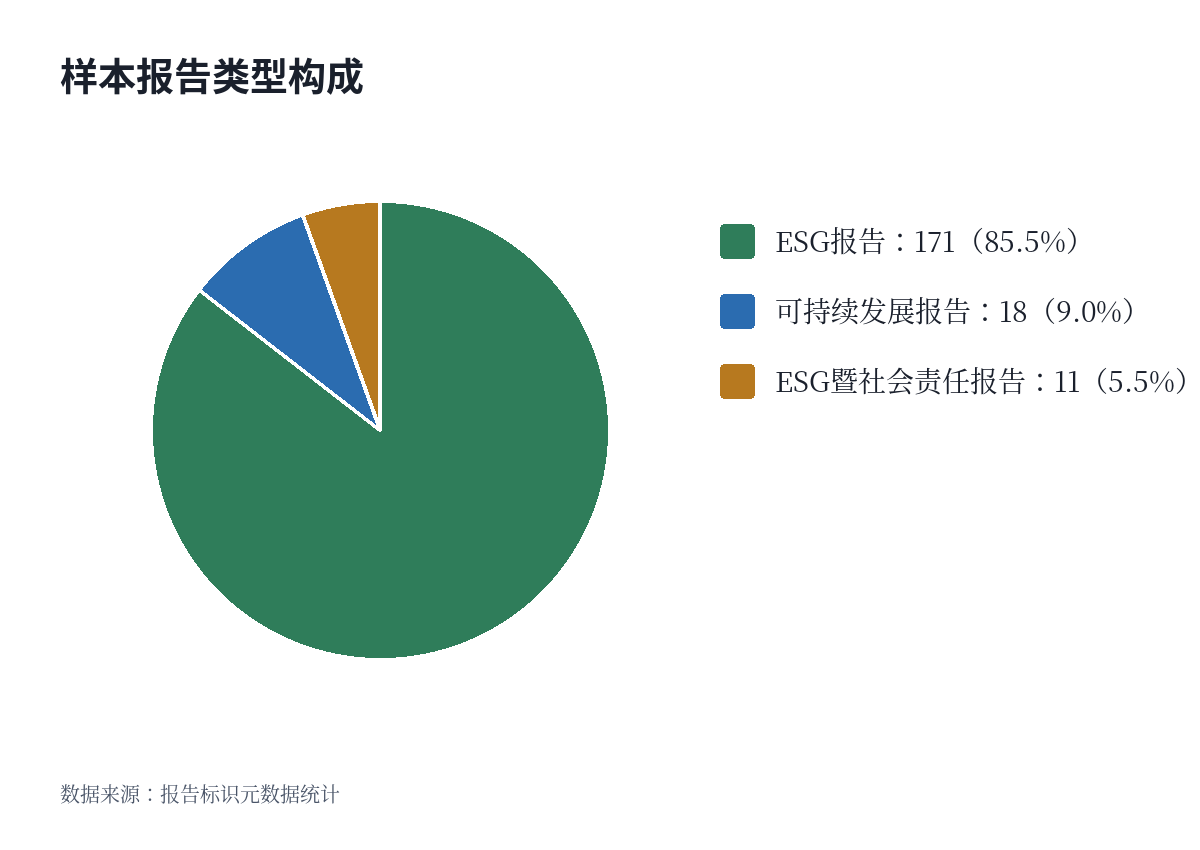
\includegraphics[width=0.86\linewidth]{fig_dataset_composition.png}
\caption{样本报告类型构成}
\label{fig:dataset-composition}
\end{figure}

\begin{figure}[htbp]
\centering
\begin{subfigure}{0.48\linewidth}
\centering
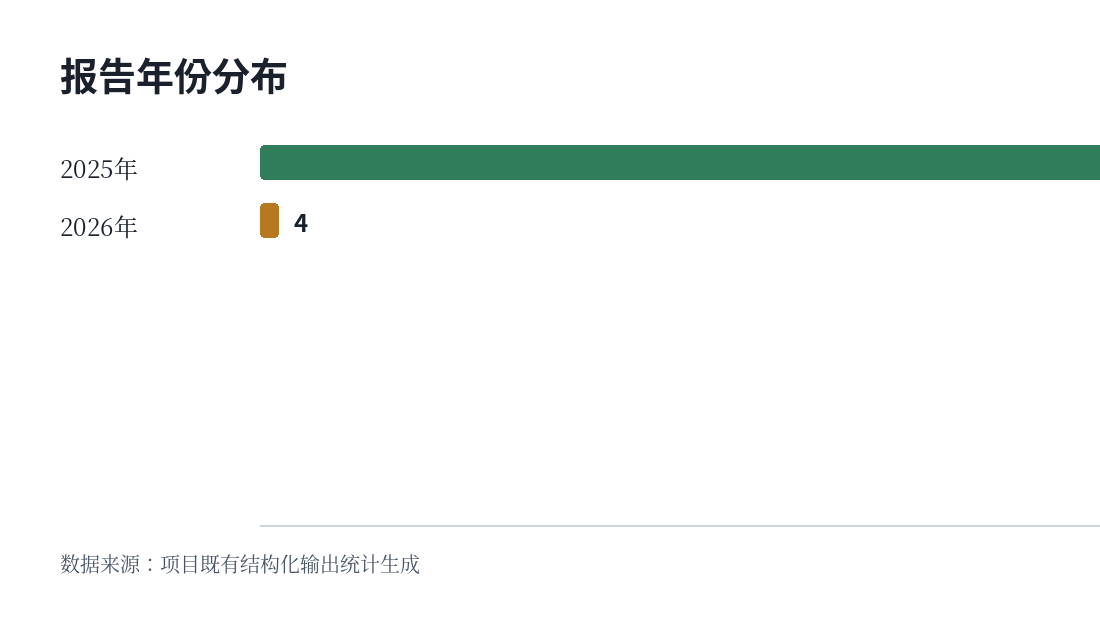
\includegraphics[width=\linewidth]{fig_year_distribution.png}
\caption{报告年份分布}
\label{fig:year-distribution}
\end{subfigure}
\begin{subfigure}{0.48\linewidth}
\centering
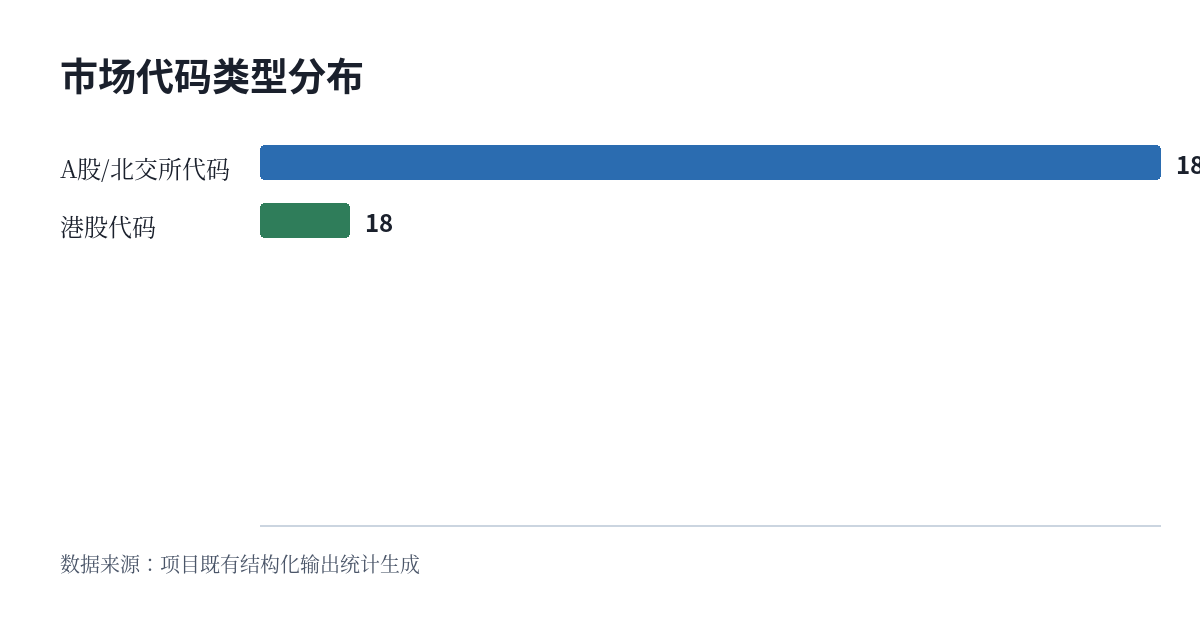
\includegraphics[width=\linewidth]{fig_market_distribution.png}
\caption{市场代码类型分布}
\label{fig:market-distribution}
\end{subfigure}
\caption{样本年份与市场代码类型分布}
\label{fig:year-market}
\end{figure}

\subsection{PDF 页数、文本与版面元素}
MinerU 解析 manifest 记录 200 份报告均形成可用 Markdown，解析成功比例为 1.0000。解析页数总计 10528 页，单份报告页数最少 1 页、最多 130 页，平均 52.64 页，中位数 51.5 页。Markdown 字符总量为 17740555，平均每份 88702.77 字符。manifest 中表格标记总数为 6713，图片引用总数为 30465，说明 ESG 报告的主体信息并非只存在于连续正文中。

\begin{figure}[htbp]
\centering
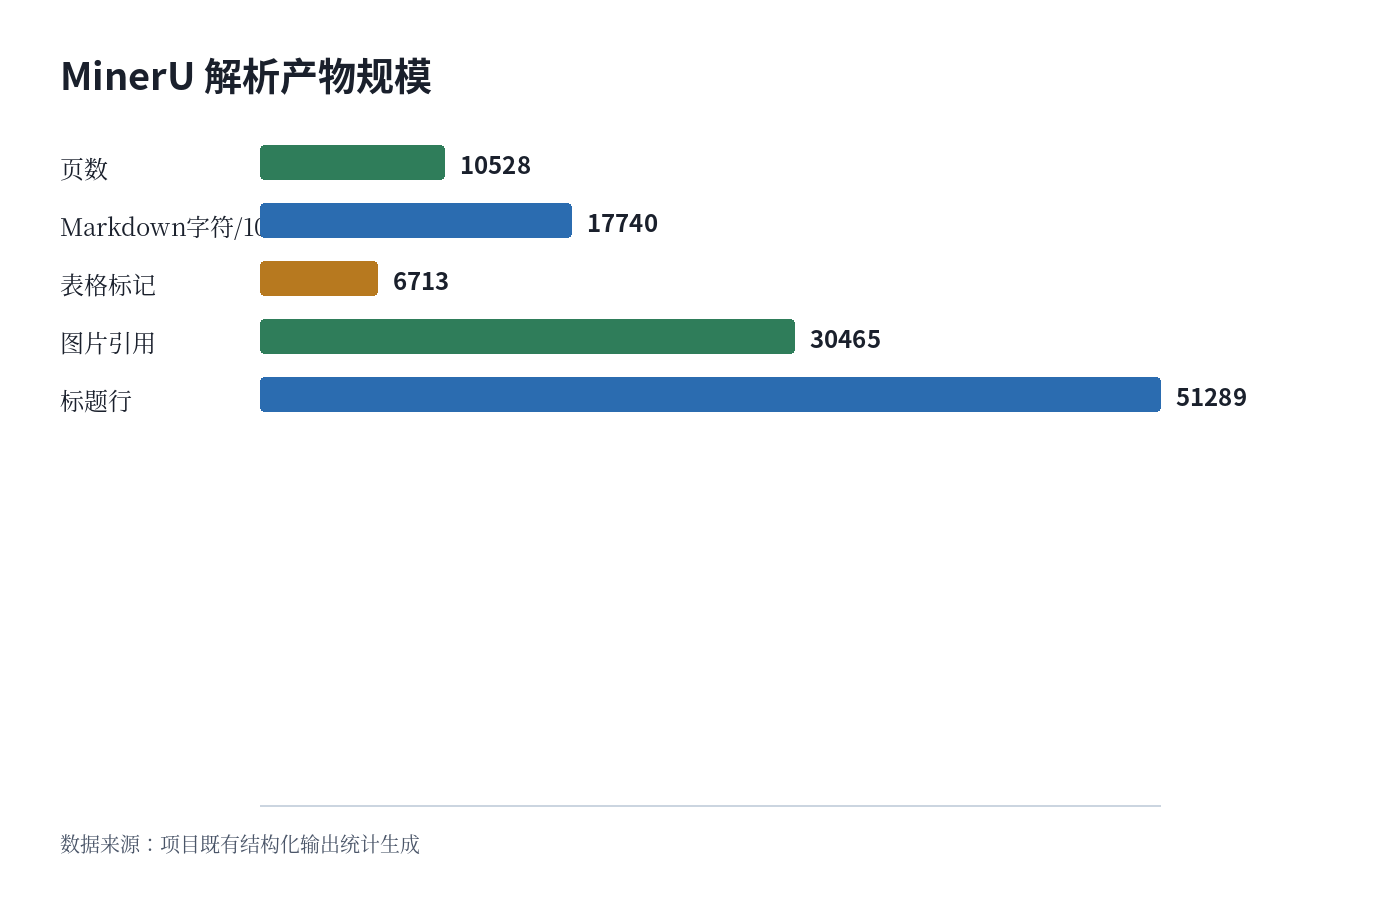
\includegraphics[width=0.92\linewidth]{fig_parse_scale.png}
\caption{MinerU 解析产物规模}
\label{fig:parse-scale}
\end{figure}

进一步展开解析后的块级结构，本文得到 235662 个内容块，平均每份报告 1178.31 个。主要块类型包括 paragraph 83390 个、title 51806 个、page\_header 42113 个、image 28123 个、page\_number 15692 个、table 6455 个。内容块数量与类型分布表明，直接把整份 PDF 输入语言模型会引入大量无关上下文，而只按关键词搜索又容易丢失表格和章节上下文。

\begin{figure}[htbp]
\centering
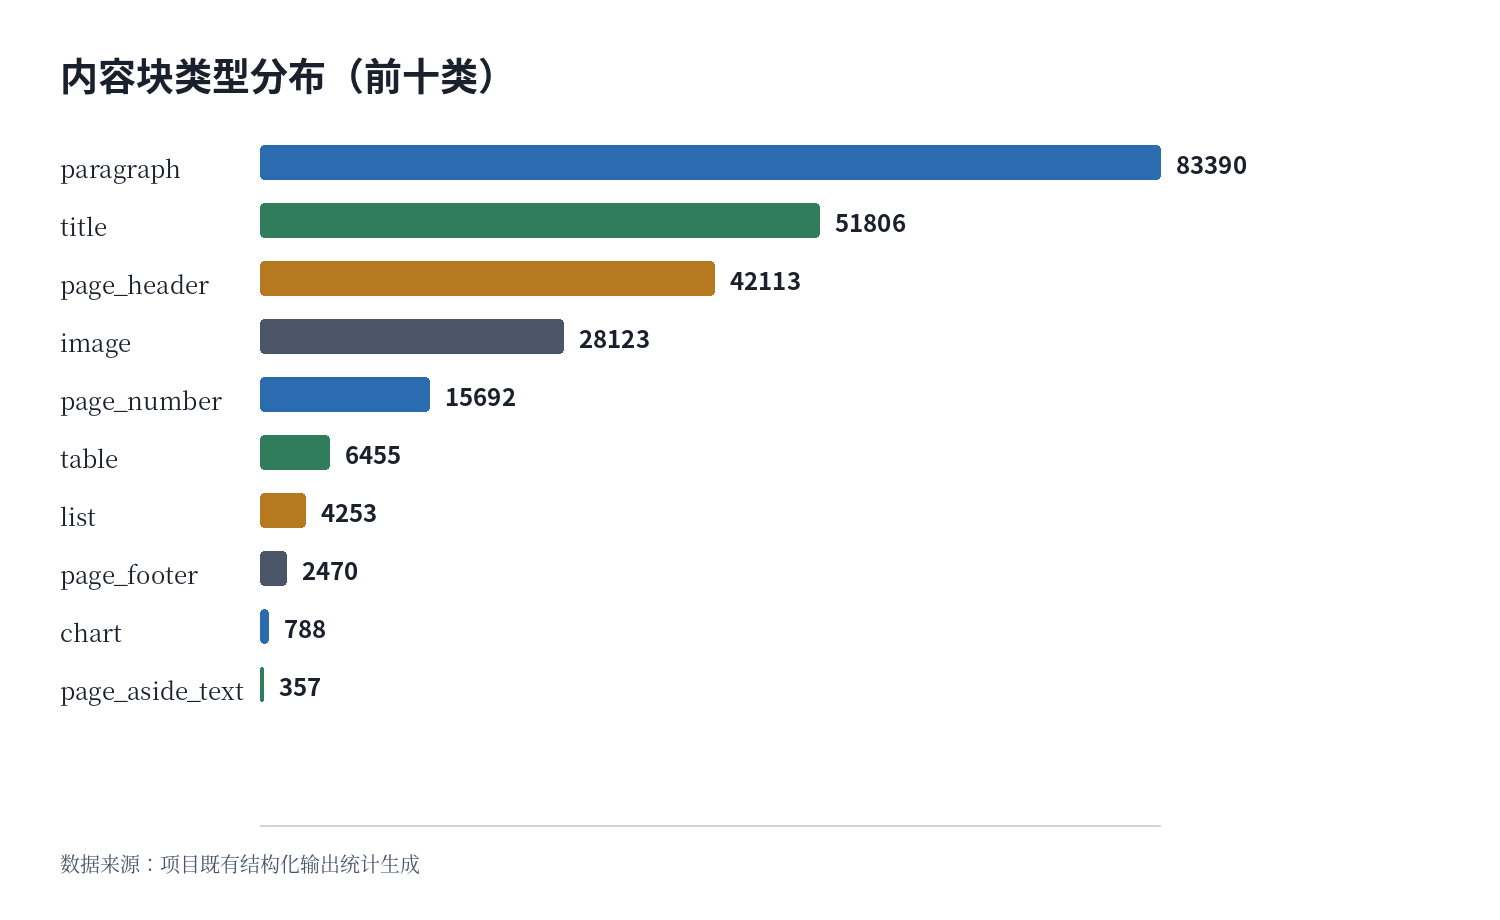
\includegraphics[width=0.95\linewidth]{fig_block_type_distribution.png}
\caption{内容块类型分布}
\label{fig:block-type}
\end{figure}

\subsection{文档特征对建模的影响}
ESG 报告的结构化难点主要来自四方面。第一，长文档中同一指标可能在目录、章节标题、正文解释、表格和附录中重复出现，证据位置需要被区分。第二，定量指标常在表格中披露，单位可能位于表头或同一行附近，value 与 unit 的绑定依赖局部上下文。第三，定性指标需要保留完整机制描述，过短证据会降低复核价值。第四，不同行业和公司披露口径不同，关键词只能提供候选线索，不能直接替代语义判断。因此本文采用“内容块建模--候选证据召回--证据约束抽取--质量诊断”的链式方法。

\newpage
\section{问题分析与建模思路}
\subsection{长文档抽取难点}
设第 $i$ 份报告为 $d_i$，其解析后的内容块集合为 $B_i$。若对整篇报告直接进行抽取，模型需要在数万字符甚至十余万字符中寻找某一指标证据，成本高且难以保证证据位置。若只使用规则抽取，则同义表述、跨表头单位、政策描述和零事件表达难以覆盖。本文将大语言模型放在候选证据范围内使用，使其承担局部语义抽取，而不承担无约束生成。

\subsection{总体技术路线}
本文技术路线如 \figref{fig:overall-pipeline} 所示。报告首先通过 MinerU 转换为 Markdown、JSON 和图片资源，再展开为带页码、块号、类型和文本的内容块序列；随后将 65 个 ESG 指标与 200 份报告组合为 13000 个 report-indicator 任务；每个任务通过关键词、单位、块类型和位置等线索召回候选证据；候选为空时直接输出 missing，候选非空时由 qwen3 在证据约束下输出 JSON；最后通过后处理、质量诊断和 Streamlit 系统形成复核闭环。

\begin{figure}[htbp]
\centering
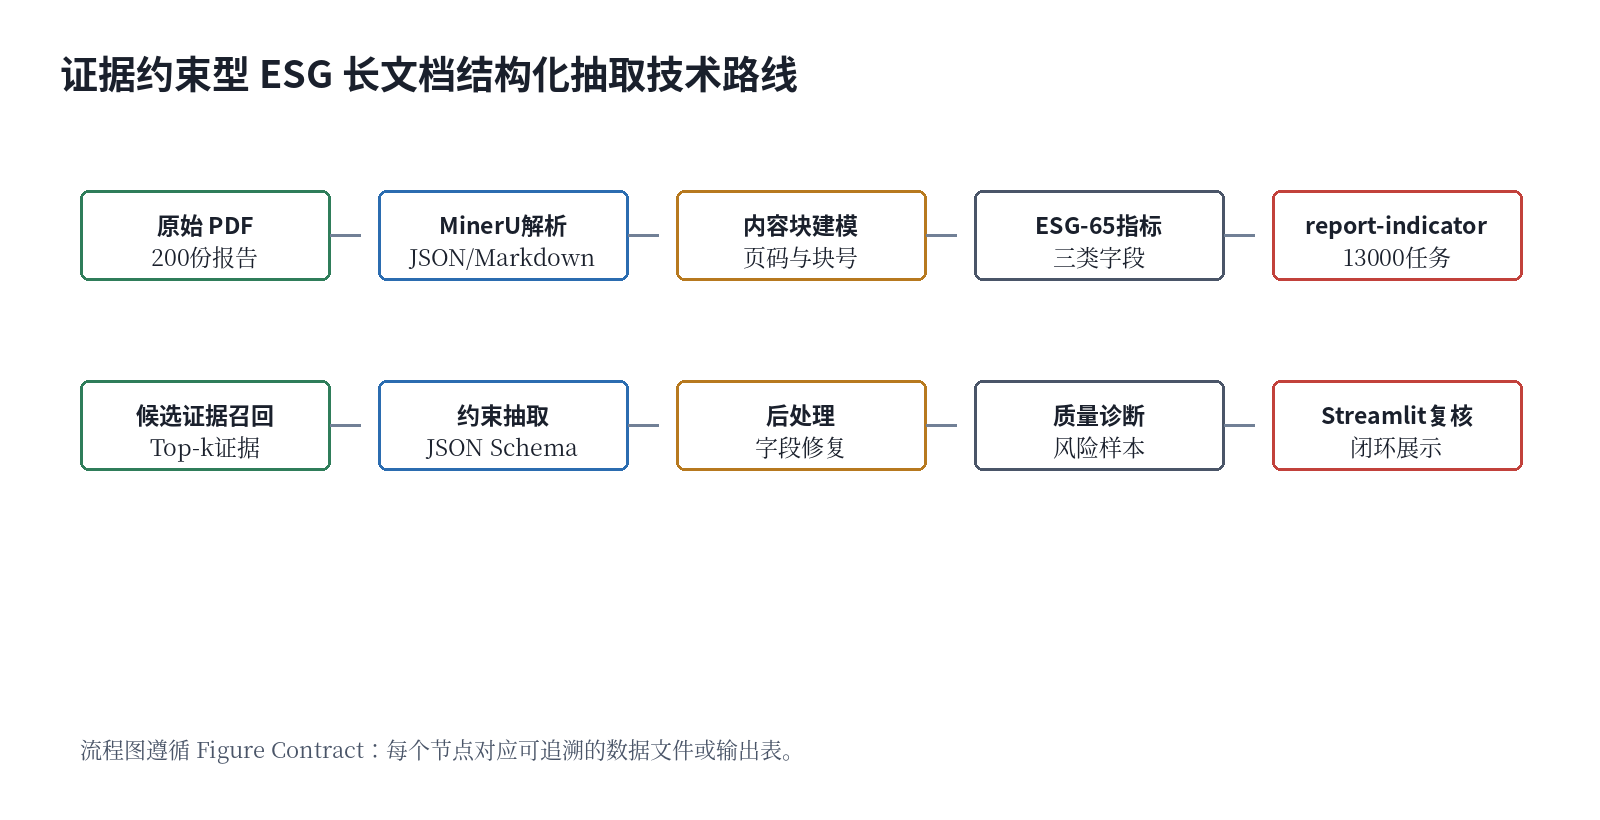
\includegraphics[width=\linewidth]{fig_overall_pipeline.png}
\caption{证据约束型 ESG 长文档结构化抽取技术路线}
\label{fig:overall-pipeline}
\end{figure}

\newpage
\section{模型假设与符号说明}
\subsection{模型假设}
本文模型建立在以下假设之上：
\begin{enumerate}
  \item 公开 ESG 报告内容可用于赛题范围内的算法验证。
  \item MinerU 解析结果能保留主要文本、表格文本、页码和块顺序。
  \item report-indicator 判断必须基于候选证据；候选证据不足时不补写结果。
  \item ESG-65 指标体系覆盖本文任务所需主要披露类型，但不声称覆盖全部 ESG 披露项。
  \item 自动质量诊断用于组织复核优先级，不等同于完整人工真值集。
  \item 本文不建立 ESG 评分、排名或投资建议模型。
\end{enumerate}

\subsection{符号说明}
\begin{table}[htbp]
\centering
\caption{主要符号说明}
\label{tab:symbols}
\begin{tabularx}{\linewidth}{llX}
\toprule
符号 & 含义 & 说明 \\
\midrule
$D$ & 报告集合 & $D=\{d_1,d_2,\ldots,d_n\}$，本文 $n=200$ \\
$d_i$ & 第 $i$ 份报告 & 原始 PDF 及其解析产物 \\
$B_i$ & 内容块集合 & 第 $i$ 份报告解析后的块序列 \\
$b_{ik}$ & 内容块 & 包含 report\_id、page\_no、block\_id、block\_type、text \\
$Q$ & 指标集合 & ESG-65 指标体系 \\
$q_j$ & 第 $j$ 个指标 & 包含维度、类型、关键词、单位候选和风险标记 \\
$K_j$ & 关键词集合 & 指标 $q_j$ 的候选召回词集合 \\
$U_j$ & 单位候选集合 & 定量指标的单位约束集合 \\
$s(b,q)$ & 候选评分 & 内容块 $b$ 对指标 $q$ 的证据相关性 \\
$E_{ij}$ & 候选证据集合 & 报告 $d_i$ 对指标 $q_j$ 的 Top-k 证据块 \\
$F$ & 证据约束抽取函数 & 在 $E_{ij}$ 范围内输出结构化记录 \\
$R_j$ & 后处理规则 & 与指标类型和风险标记相关的字段检查规则 \\
$y_{ij}$ & 输出记录 & report-indicator 结构化结果 \\
\bottomrule
\end{tabularx}
\end{table}

\newpage
\section{模型建立}
\subsection{PDF 结构化解析与内容块表示}
PDF 不是天然面向结构化抽取的数据格式，文档智能研究通常需要先处理版面分析、表格抽取和内容顺序恢复等问题\parencite{zhong2019publaynet,smock2022pubtables}。本文使用 MinerU 将 PDF 转换为 JSON、Markdown 和图片资源\parencite{cui2025mineru}，其中 Markdown 便于文本检索，JSON 保留块级结构，图片资源保留图表和版面证据。每个内容块定义为
\begin{equation}
b_{ik}=(report\_id,page\_no,block\_id,block\_type,text),
\end{equation}
第 $i$ 份报告的证据空间表示为
\begin{equation}
B_i=\{b_{i1},b_{i2},\ldots,b_{im_i}\}.
\end{equation}
表格块对定量指标尤其重要，因为 value 与 unit 往往在同一表格行、列标题或相邻单元格中出现。标题块和段落块则更多服务于定性、机制性指标的证据定位。

\begin{figure}[htbp]
\centering
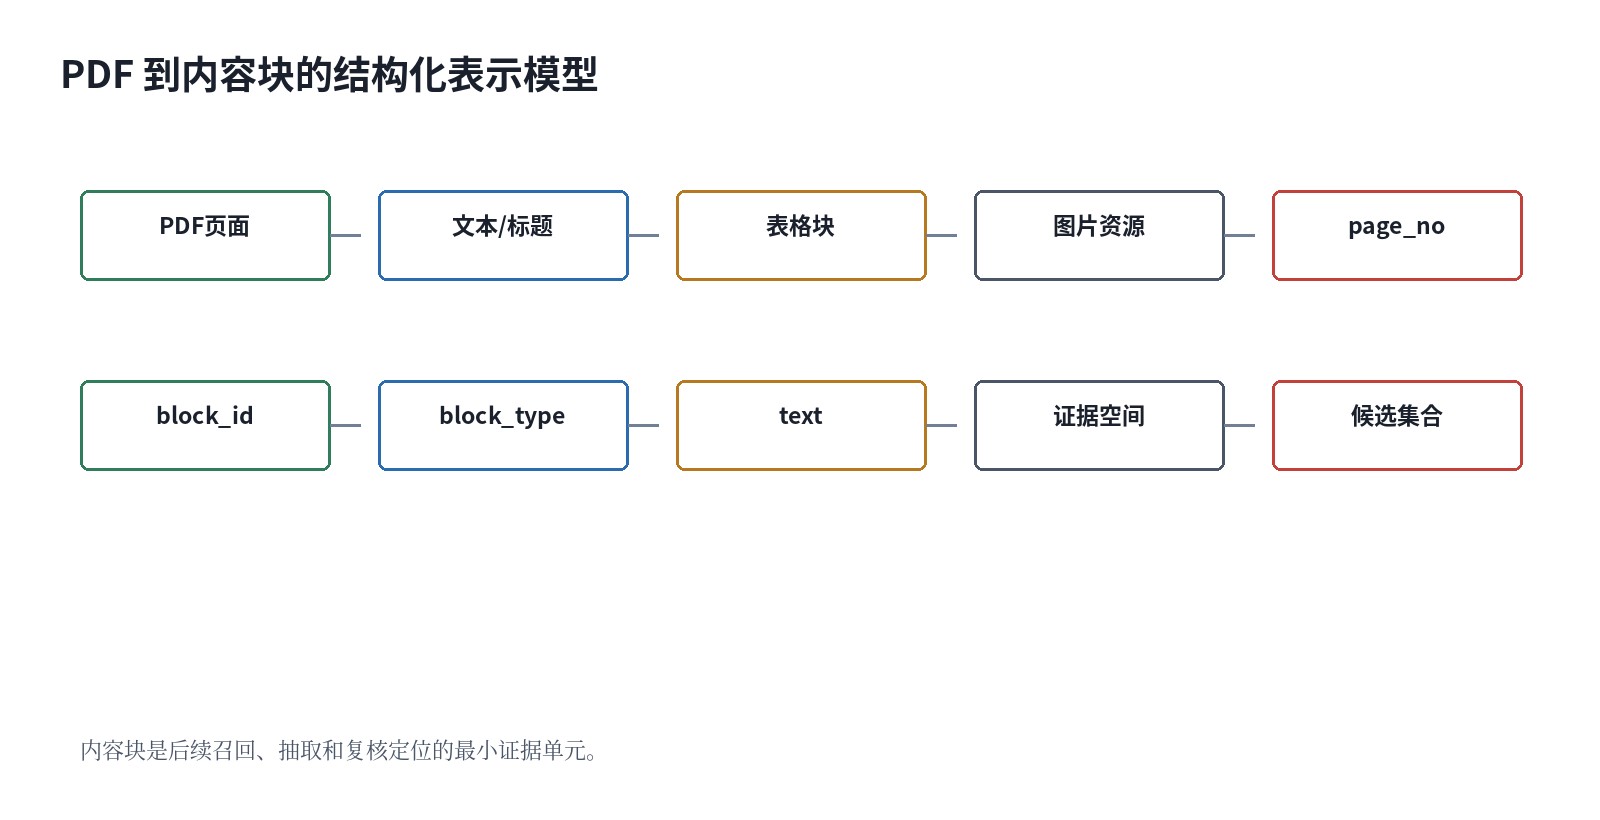
\includegraphics[width=\linewidth]{fig_block_model.png}
\caption{PDF 到内容块的结构化表示模型}
\label{fig:block-model}
\end{figure}

\subsection{ESG-65 指标体系建模}
指标体系 $Q$ 由赛题要求、ESG 报告高频披露项和前序质检结果共同约束，包含 E 维度 25 个、S 维度 20 个、G 维度 20 个；按类型划分，定量指标 35 个、机制性布尔指标 15 个、定性描述指标 15 个。每个指标表示为
\begin{equation}
q_j=(id_j,name_j,dim_j,type_j,K_j,U_j,risk_j).
\end{equation}
其中 $K_j$ 为关键词集合，$U_j$ 为单位候选集合，$risk_j$ 用于标记需重点复核的指标或字段。定量指标输出 value 和 unit，定性指标输出 qualitative\_text，机制性布尔指标输出 true/false 与原文机制证据。

\begin{table}[htbp]
\centering
\caption{ESG-65 指标体系维度分布}
\label{tab:indicator-summary}
\begin{tabular}{lllll}
\toprule
项目 & E & S & G & 合计 \\
\midrule
指标数 & 25 & 20 & 20 & 65 \\
\bottomrule
\end{tabular}

\end{table}

\begin{figure}[htbp]
\centering
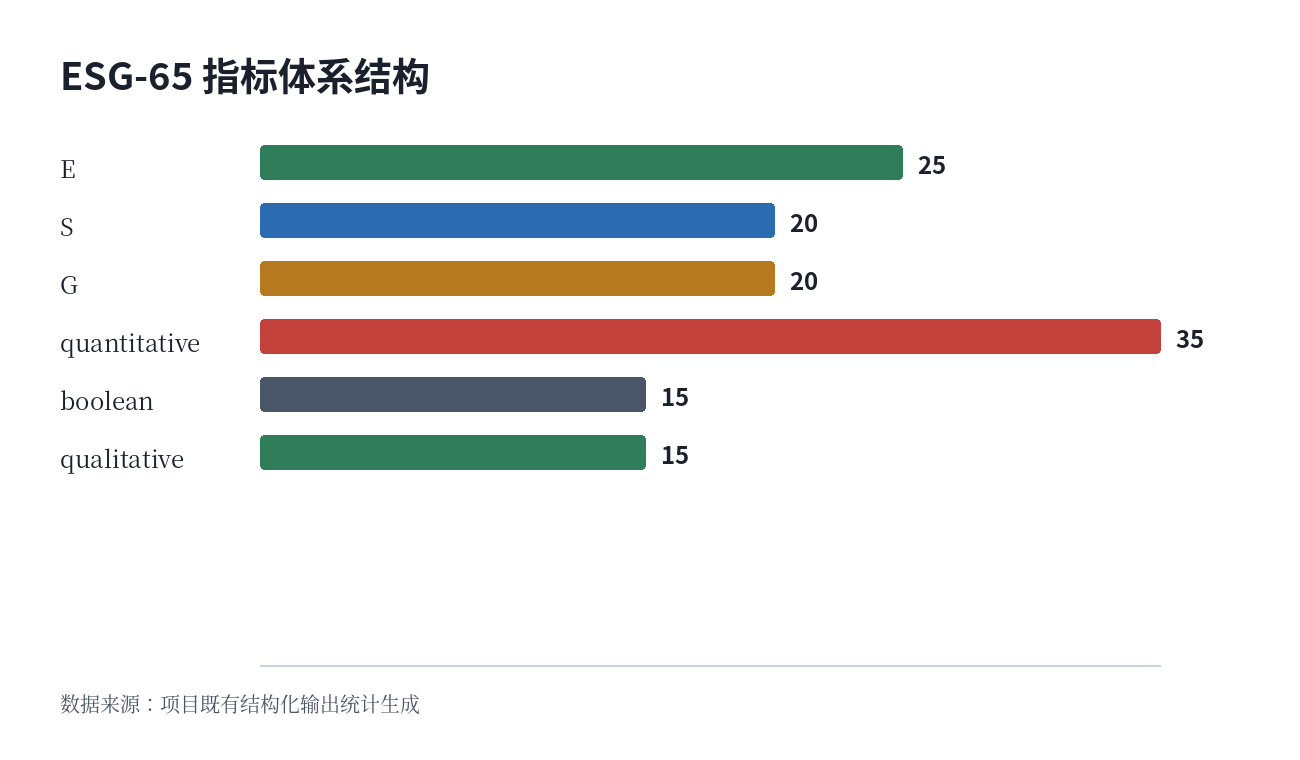
\includegraphics[width=0.92\linewidth]{fig_indicator_system.png}
\caption{ESG-65 指标体系结构}
\label{fig:indicator-system}
\end{figure}

\subsection{report-indicator 任务定义}
对每份报告 $d_i$ 和每个指标 $q_j$ 构造一个任务，输出结构化记录
\begin{equation}
\begin{aligned}
y_{ij}=(&status,value,unit,qualitative\_text,\\
        &evidence\_quote,page\_no,block\_id,risk\_tag).
\end{aligned}
\end{equation}
其中 $status \in \{found,missing,error\}$。found 表示在候选证据约束下生成了结构化字段，missing 表示当前证据不足以支持该指标披露，error 表示流程异常。该状态集合描述自动抽取流程的运行输出，不表示人工标注评价结论。

\subsection{候选证据召回模型}
候选召回的目标是在长文档中缩小语义抽取范围。对内容块 $b$ 与指标 $q$，定义候选评分
\begin{equation}
s(b,q)=w_k\,match_K(b,q)+w_u\,match_U(b,q)+w_t\,type\_score(b)+w_p\,position\_score(b).
\end{equation}
$match_K$ 衡量关键词命中，$match_U$ 衡量单位候选命中，$type\_score$ 对表格、段落和标题等块类型赋予差异权重，$position\_score$ 反映标题邻近、章节上下文和块序位置等线索。每个任务选择 Top-k 内容块构成 $E_{ij}$。当 $E_{ij}$ 为空时，流程直接输出 missing；当 $E_{ij}$ 非空时，才进入模型抽取链路。该设计降低了长文档噪声，也减少了模型调用规模。

\begin{figure}[htbp]
\centering
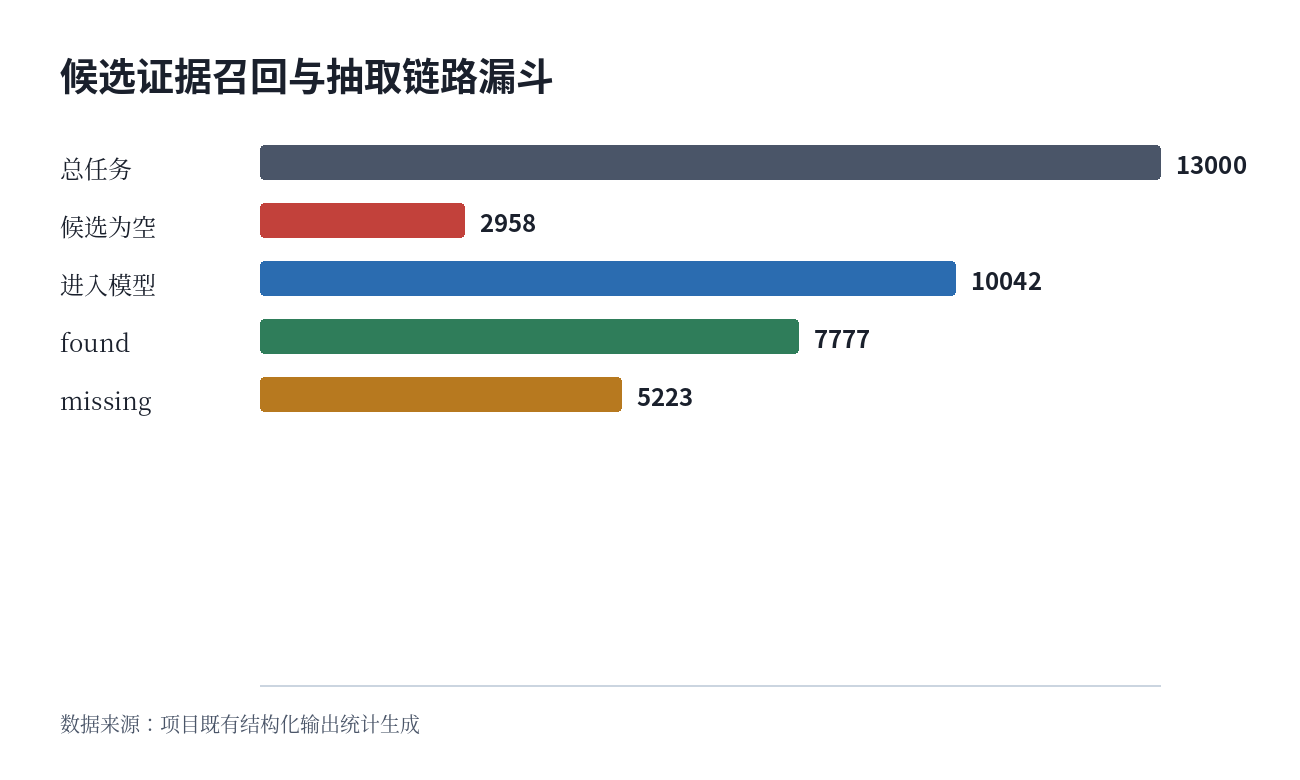
\includegraphics[width=0.92\linewidth]{fig_candidate_funnel.png}
\caption{候选证据召回与抽取链路漏斗}
\label{fig:candidate-funnel}
\end{figure}

\subsection{大语言模型证据约束抽取模型}
本文使用 qwen3 作为候选证据范围内的语义抽取器，调用方式通过本地 Ollama 服务完成\parencite{bai2023qwen,ollama}。这一设计与检索增强生成思想相近\parencite{lewis2020rag}，但本文的重点不是开放式生成，而是在局部候选证据内输出可复核字段。模型输入由当前 report-indicator 任务、指标定义和候选证据组成，不使用报告外知识。抽取约束包括：证据不足必须 missing；定量 found 必须包含 value 和 unit；定性 found 保留原文语义片段；机制性布尔 found 必须有制度、措施或治理安排证据；evidence\_quote 必须来自候选证据；输出必须符合固定 JSON schema。

\begin{figure}[htbp]
\centering
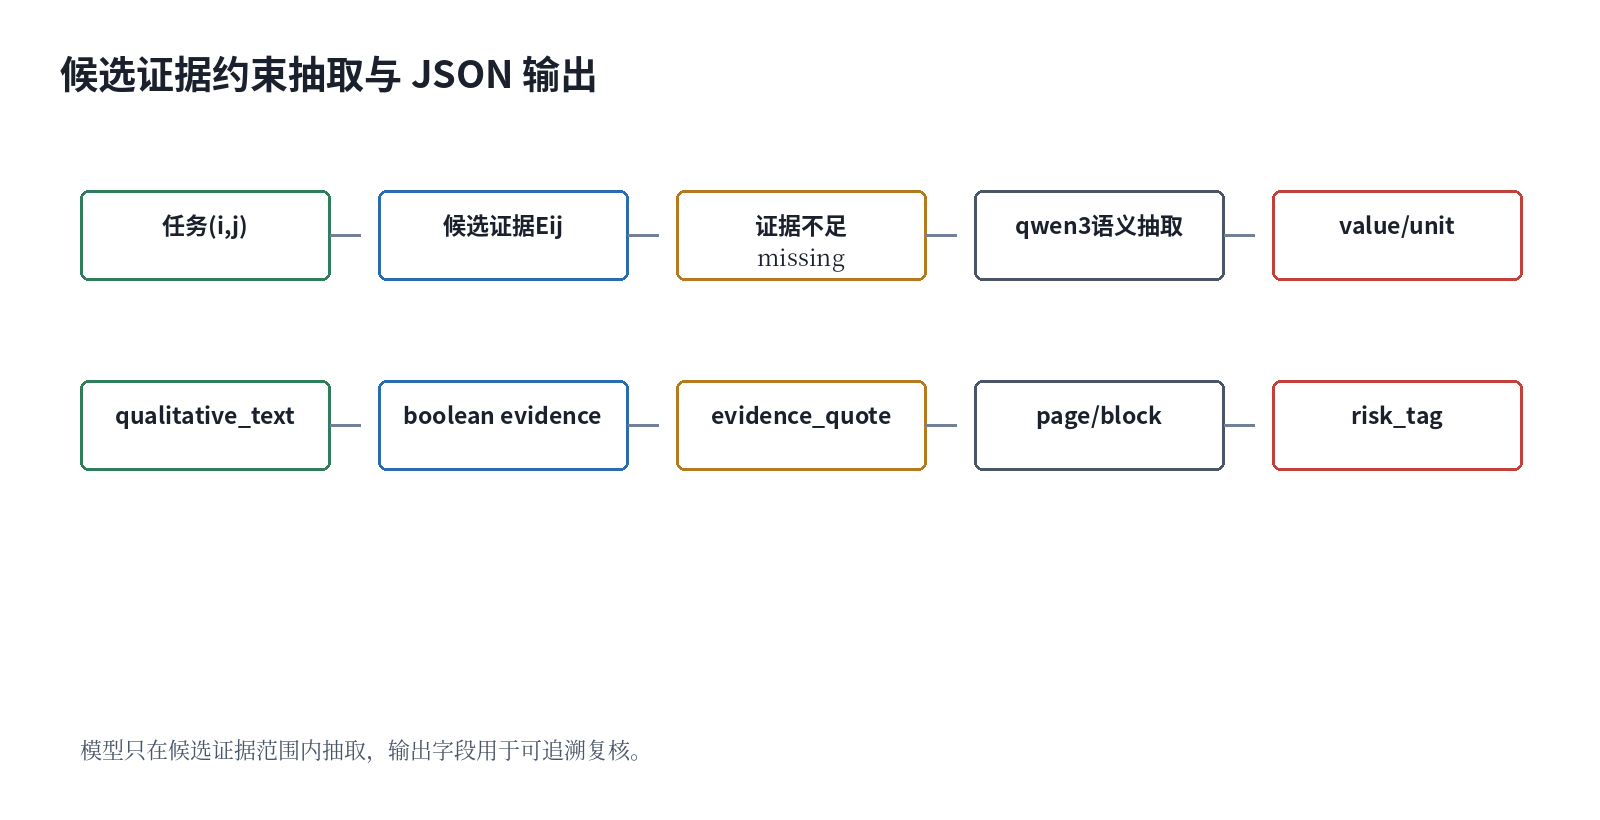
\includegraphics[width=\linewidth]{fig_extraction_schema.png}
\caption{候选证据约束抽取与 JSON 输出}
\label{fig:extraction-schema}
\end{figure}

\subsection{后处理规则与质量诊断模型}
模型输出后，系统进行 JSON 解析、字段补齐、value/unit 检查、单位修复、零事件归一和风险标记。质量诊断不把样本判为最终对错，而是识别复核优先级。风险类型包括 value/unit 缺失、比例误作数量、金额误作数量、零事件归一、证据过短和标题式机制证据。risk\_tag 记录具体触发规则，risk\_level 用 high、medium、low 表示复核优先级，caution\_tag 用于提示高风险指标或需要人工关注的样本。

\begin{figure}[htbp]
\centering
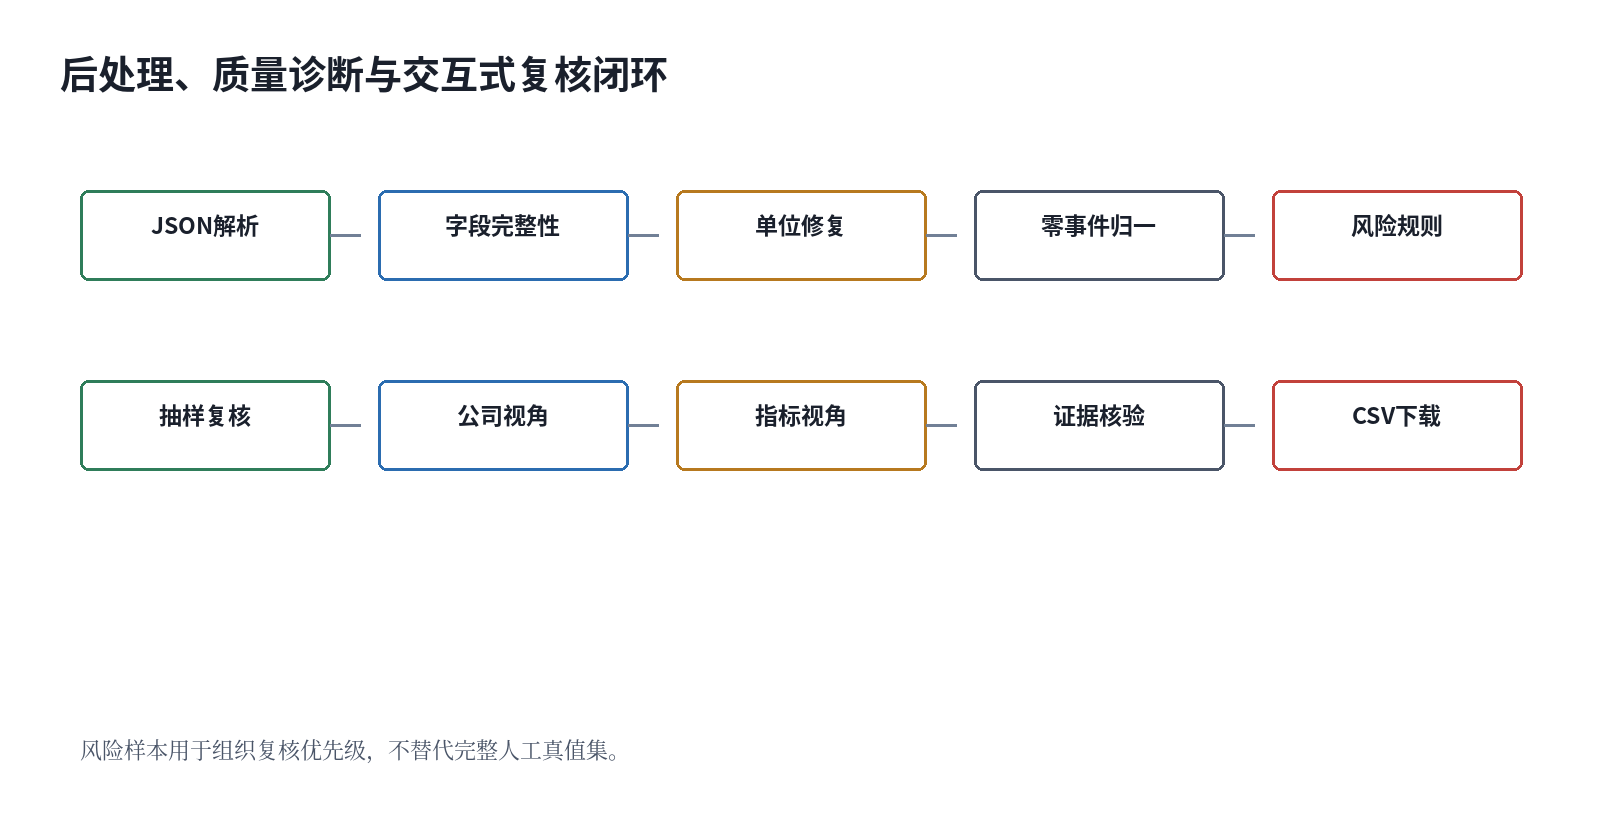
\includegraphics[width=\linewidth]{fig_quality_loop.png}
\caption{后处理、质量诊断与交互式复核闭环}
\label{fig:quality-loop}
\end{figure}

\subsection{交互式复核系统设计}
Streamlit 系统不是附属截图，而是结构化结果的复核出口\parencite{streamlit}。系统数据源为结构化 JSON，提供系统总览、公司视角、指标视角、证据核验、高风险样本和新报告接入六个页面。公司视角用于查看单份报告的 65 个指标结果，指标视角用于横向比较同一指标在 200 份报告中的披露情况，证据核验页面绑定 evidence\_quote、page\_no 和 block\_id，高风险样本页面用于集中处理 risk\_tag 与 risk\_level，下载功能支持将筛选结果导出为 CSV。

\begin{figure}[htbp]
\centering
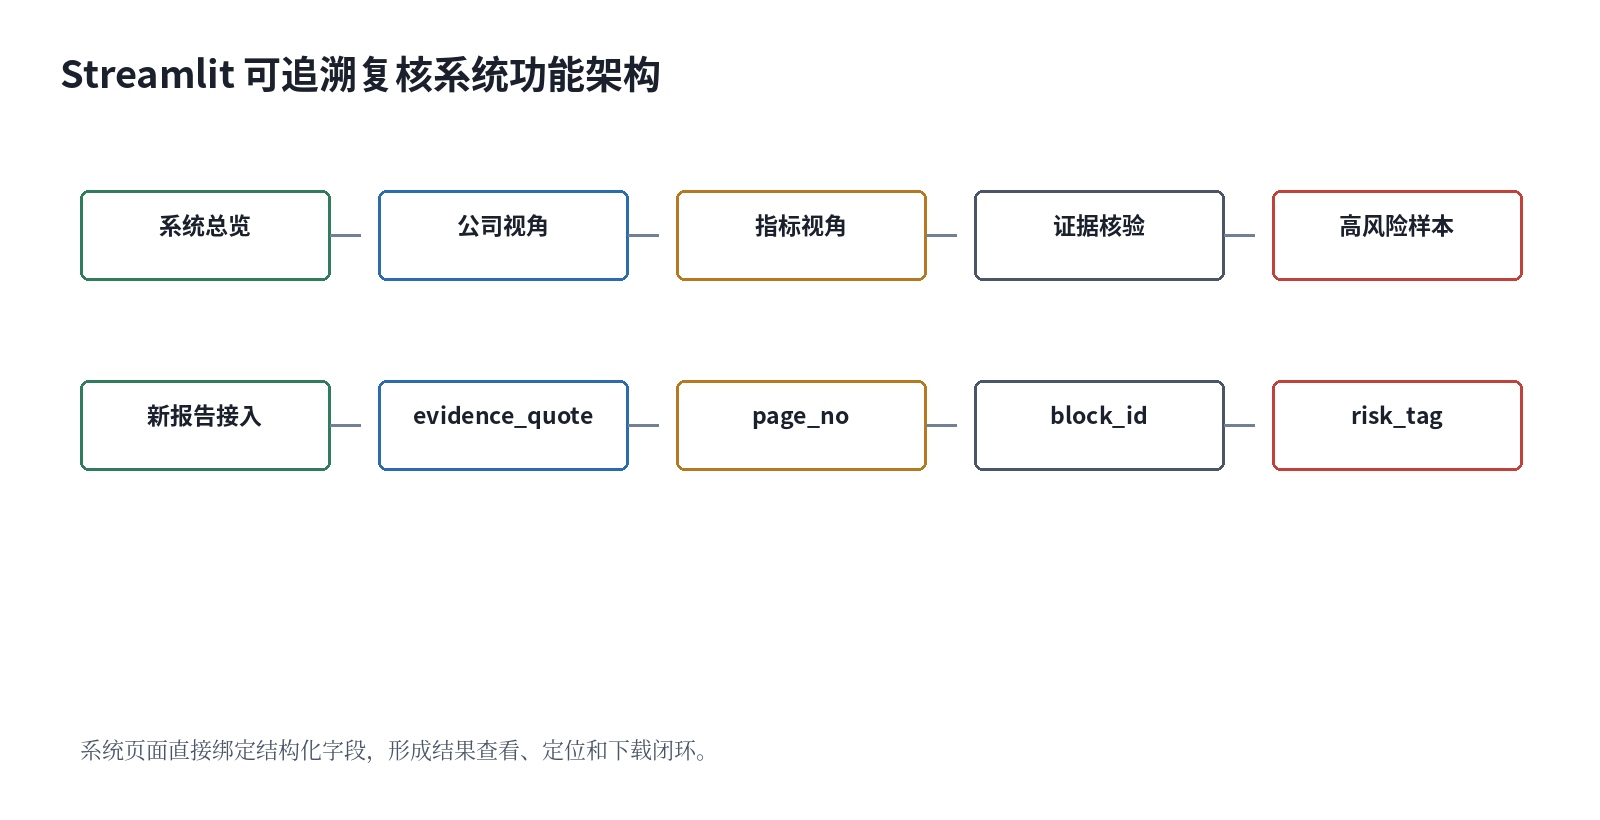
\includegraphics[width=\linewidth]{fig_streamlit_architecture.png}
\caption{Streamlit 可追溯复核系统功能架构}
\label{fig:streamlit-architecture}
\end{figure}

\begin{figure}[htbp]
\centering
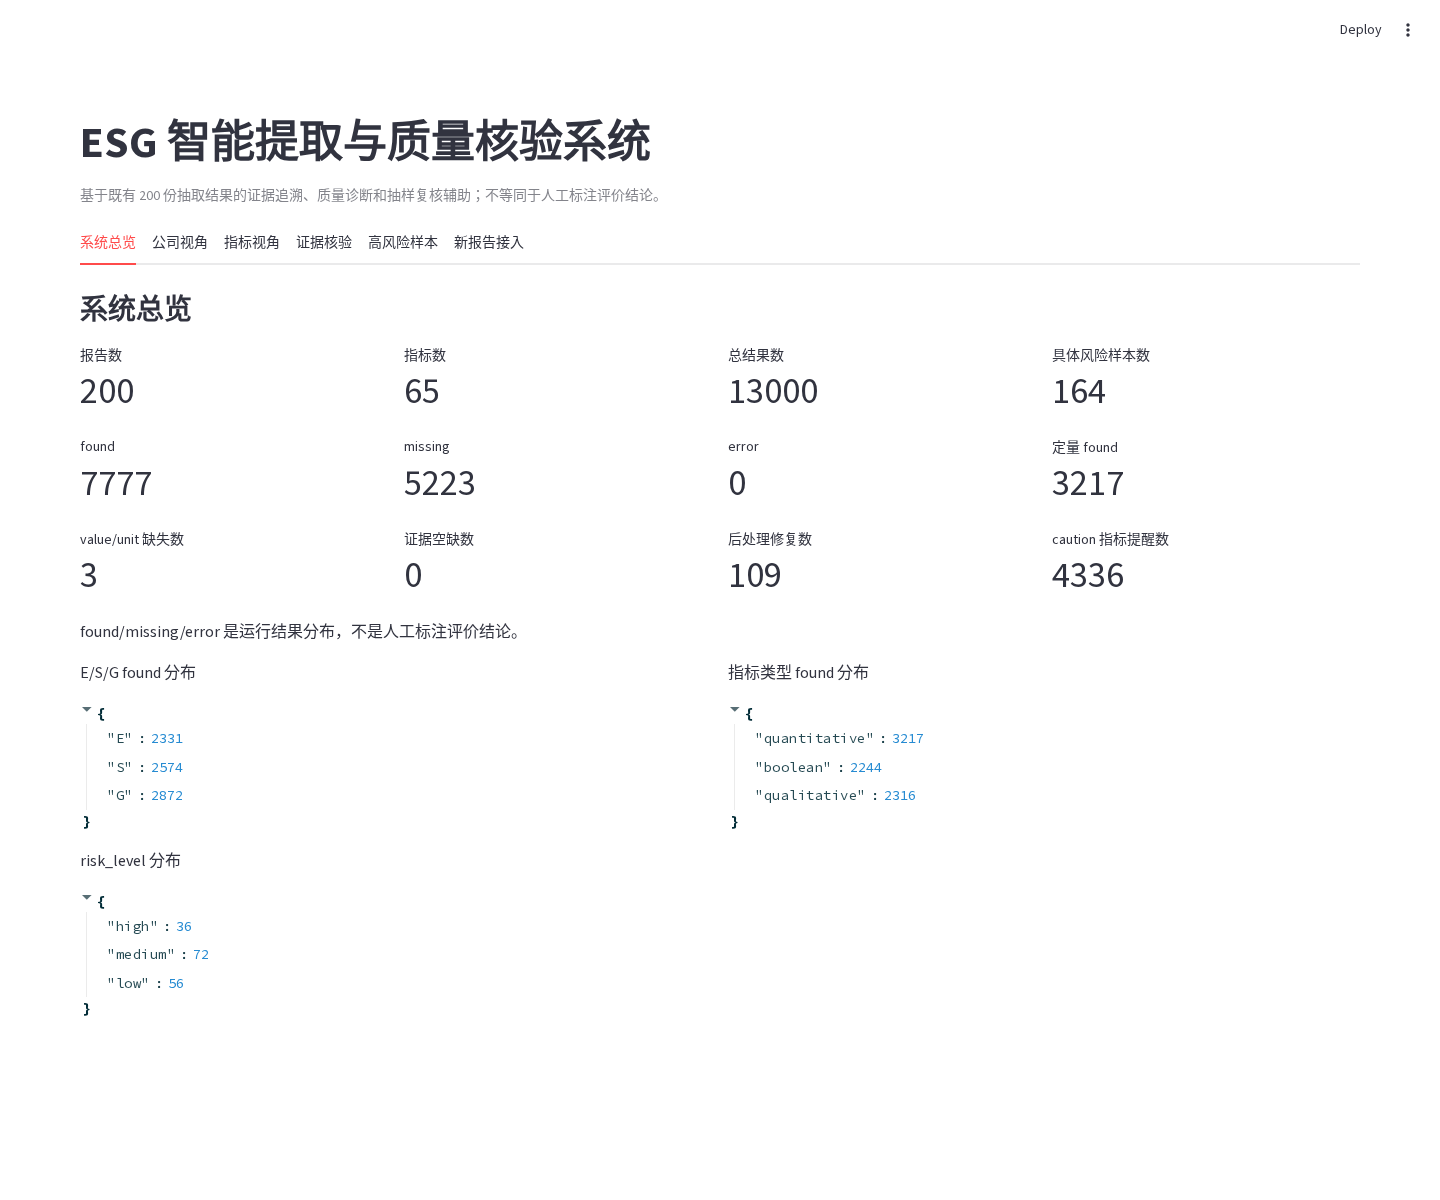
\includegraphics[width=\linewidth]{fig_system_ui_overview.png}
\caption{Streamlit 系统总览页面截图}
\label{fig:system-ui-overview}
\end{figure}

\begin{figure}[htbp]
\centering
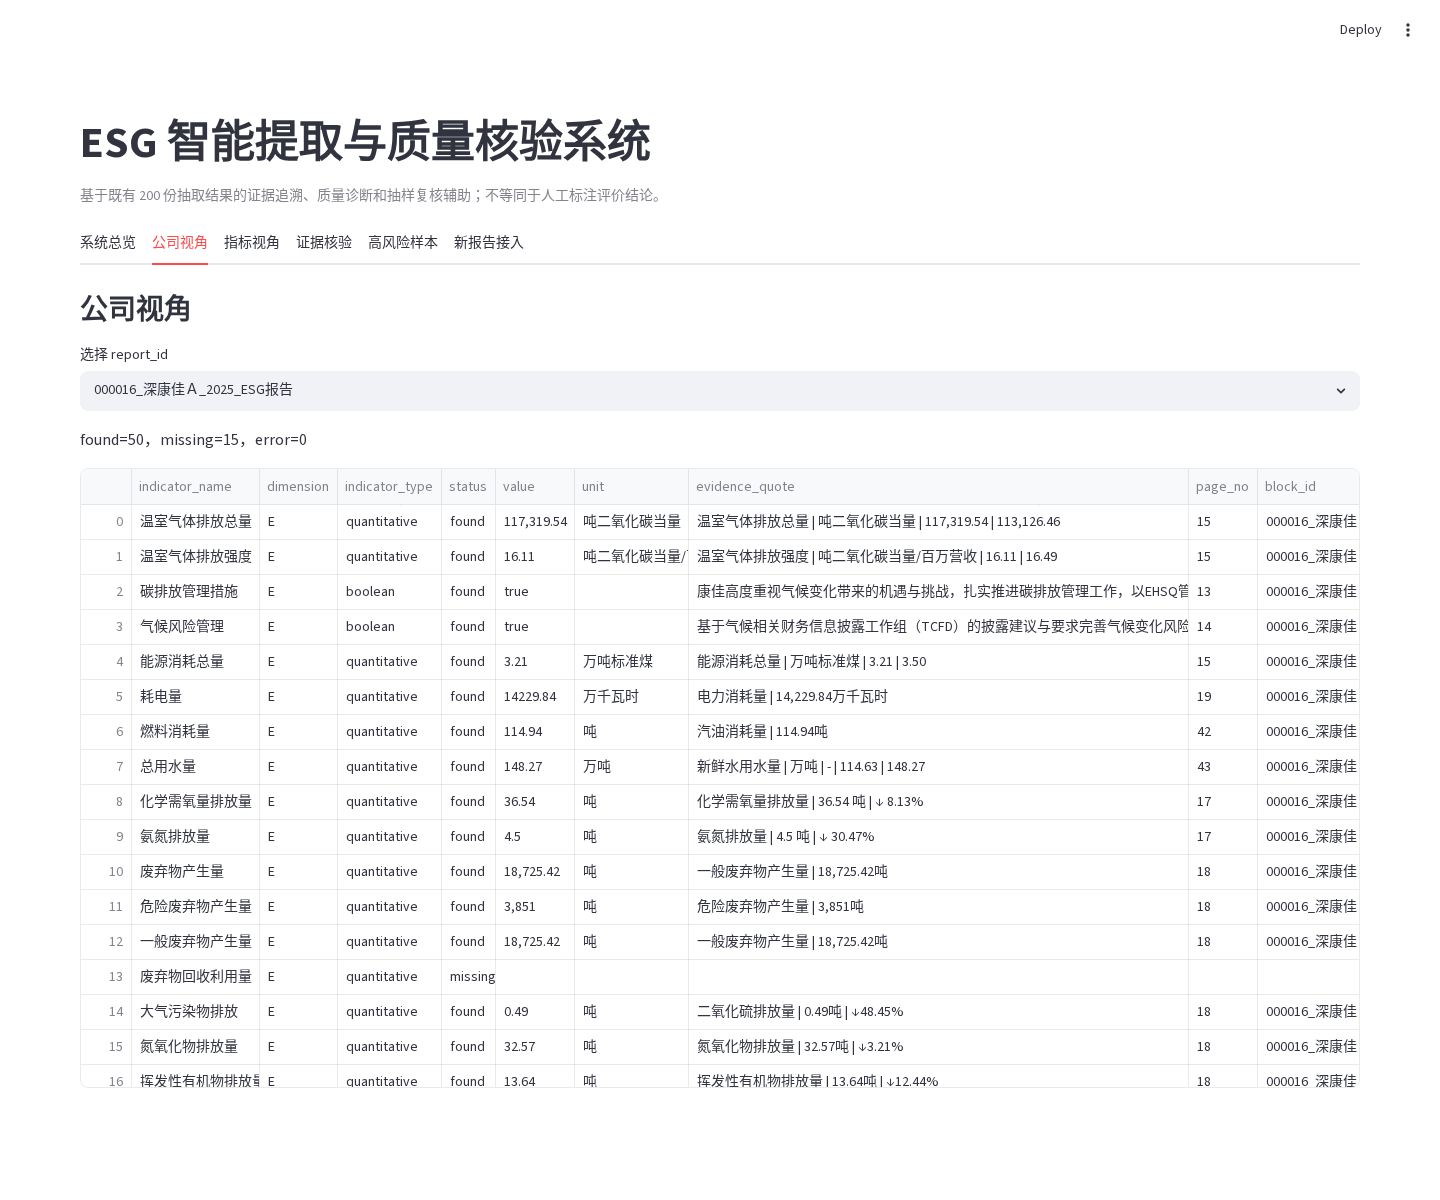
\includegraphics[width=\linewidth]{fig_system_ui_company.png}
\caption{Streamlit 公司视角页面截图}
\label{fig:system-ui-company}
\end{figure}

\begin{figure}[htbp]
\centering
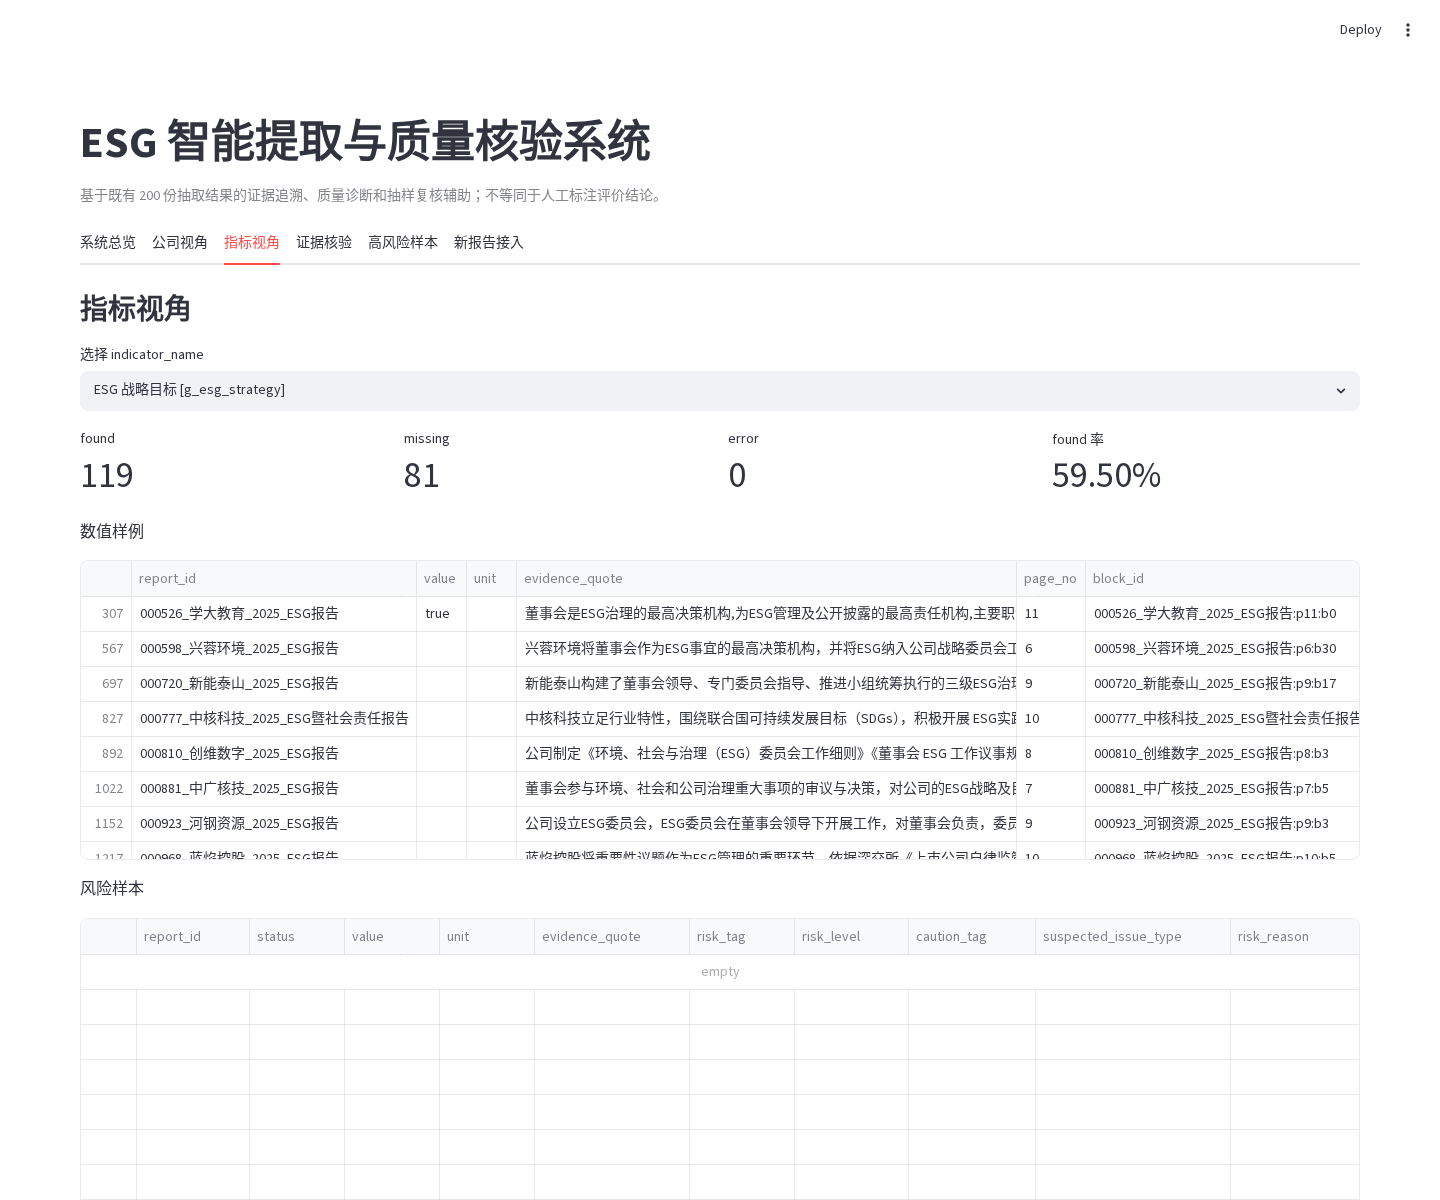
\includegraphics[width=\linewidth]{fig_system_ui_indicator.png}
\caption{Streamlit 指标视角页面截图}
\label{fig:system-ui-indicator}
\end{figure}

\begin{figure}[htbp]
\centering
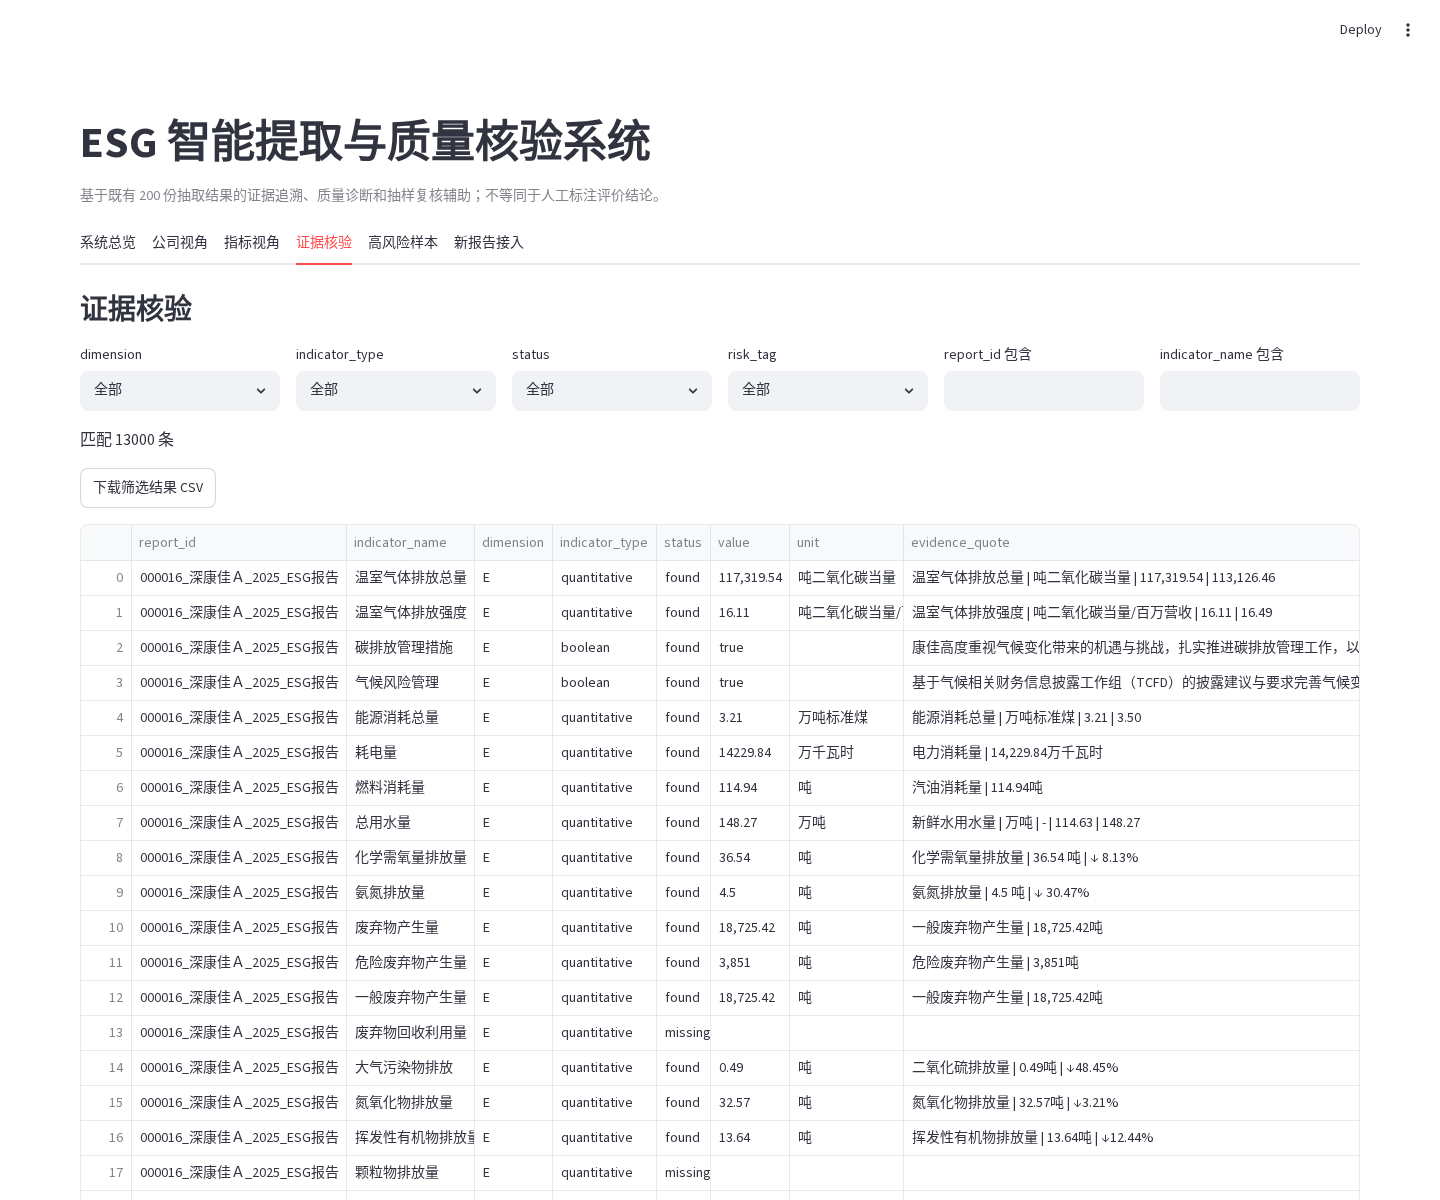
\includegraphics[width=\linewidth]{fig_system_ui_evidence.png}
\caption{Streamlit 证据核验页面截图}
\label{fig:system-ui-evidence}
\end{figure}

\begin{figure}[htbp]
\centering
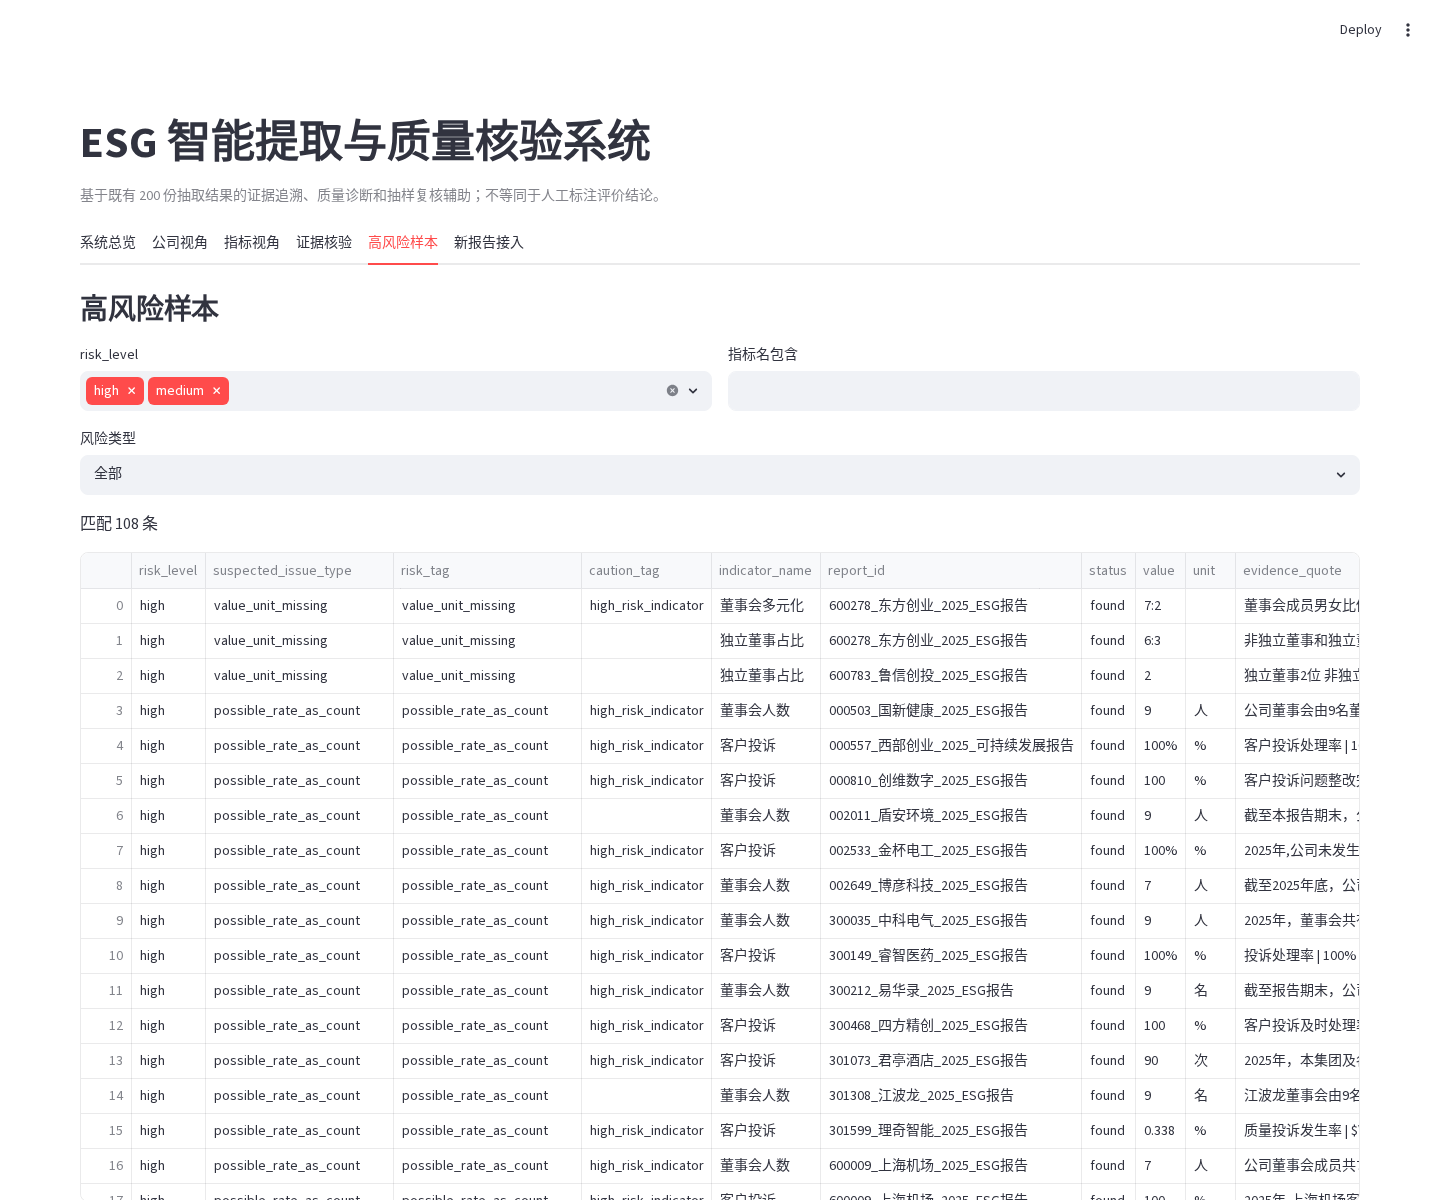
\includegraphics[width=\linewidth]{fig_system_ui_risk.png}
\caption{Streamlit 高风险样本页面截图}
\label{fig:system-ui-risk}
\end{figure}

\newpage
\section{模型求解与实现}
\subsection{求解流程}
模型求解过程由四个阶段组成。第一阶段是块级证据空间构造，将报告解析结果统一表示为有序内容块集合 $B_i$；第二阶段是任务展开，将每份报告与 ESG-65 指标逐一组合为 report-indicator 任务；第三阶段是证据召回与约束抽取，先用 $s(b,q)$ 选择候选证据，再在候选证据范围内完成结构化字段抽取；第四阶段是后处理和质量诊断，对字段完整性、证据长度、单位语境和机制性证据进行规则检查。

\begin{table}[htbp]
\centering
\caption{模型求解阶段与输入输出}
\label{tab:module}
\begin{tabularx}{\linewidth}{p{2.6cm}p{3.1cm}p{3.1cm}X}
\toprule
阶段 & 输入 & 输出 & 建模作用 \\
\midrule
内容块表示 & PDF 解析文本、表格、页码 & $B_i=\{b_{i1},\ldots,b_{im_i}\}$ & 将长文档转化为可定位证据空间 \\
指标任务展开 & 报告集合 $D$、指标集合 $Q$ & $(d_i,q_j)$ 任务集合 & 明确每份报告对每个指标的抽取目标 \\
候选证据召回 & 内容块 $B_i$、指标 $q_j$ & 候选集合 $E_{ij}$ & 降低长文档噪声，限定模型上下文 \\
约束抽取 & 任务定义、候选证据 & 结构化记录 $y_{ij}$ & 输出状态、数值、单位、证据和定位字段 \\
质量诊断 & 结构化记录与证据字段 & 风险标签与复核优先级 & 标记字段缺失、证据不足和语境误用风险 \\
\bottomrule
\end{tabularx}
\end{table}

\subsection{批量求解策略}
批量求解对每份报告遍历全部指标。若候选证据为空，则记录 missing 并保留候选数；若候选非空，则进入证据约束抽取，解析 JSON，执行字段归一和后处理。异常情况包括 JSON 解析失败、字段缺失、证据为空、value/unit 不完整和模型返回异常；对应样本进入 error 或风险诊断链路。正式批次中 error 为 0，说明该批次未出现未恢复的流程异常。

\newpage
\section{实验结果与分析}
\subsection{全量抽取结果}
全量求解得到 13000 条 report-indicator 记录，对应 200 份报告与 65 个指标。运行结果中 found 7777 条、missing 5223 条、error 0 条；候选为空直接 missing 的任务为 2958 条，候选非空并进入模型判断链路的任务为 10042 条。found 样本中 page\_no 缺失 0 条、block\_id 缺失 0 条，说明可追溯定位字段在 found 结果中保持完整。

\begin{table}[htbp]
\centering
\caption{全量抽取结果摘要}
\label{tab:result-summary}
\begin{tabular}{ll}
\toprule
项目 & 数值 \\
\midrule
report-indicator 任务 & 13000 \\
found & 7777 \\
missing & 5223 \\
error & 0 \\
候选为空直接 missing & 2958 \\
进入模型判断链路 & 10042 \\
后处理修复 & 109 \\
具体风险样本 & 164 \\
\bottomrule
\end{tabular}

\end{table}

\begin{figure}[htbp]
\centering
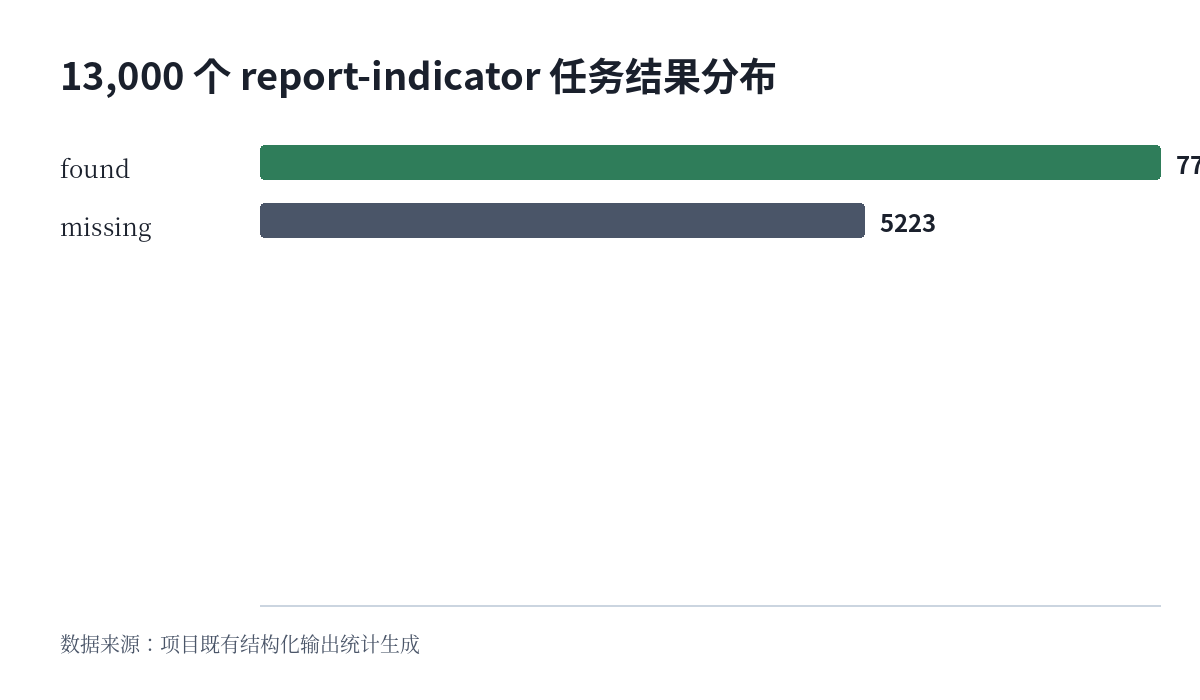
\includegraphics[width=0.86\linewidth]{fig_result_status.png}
\caption{13,000 个 report-indicator 任务结果分布}
\label{fig:result-status}
\end{figure}

\subsection{E/S/G 维度结果分析}
任务构成中 E 维度 5000 条，S 维度 4000 条，G 维度 4000 条；found 分布为 E 维度 2331 条、S 维度 2574 条、G 维度 2872 条。G 维度 found 数较高，主要因为治理结构、董事会、审计、反腐败等内容往往以固定章节和制度性表述出现，关键词召回更容易获得完整段落证据。S 维度位于中间，员工权益、供应链管理和公益投入等指标常见于社会责任章节，但员工培训、工伤、安全投入等定量指标仍依赖表格和单位。E 维度 found 数较低，并不意味着企业环境披露质量较差，而是因为 E 维度定量指标更多，且污染物、能源、水耗、废弃物等指标在不同行业中披露口径差异大；当报告只给出政策表述或未给出单位化数值时，证据约束模型会更倾向输出 missing。

\begin{figure}[htbp]
\centering
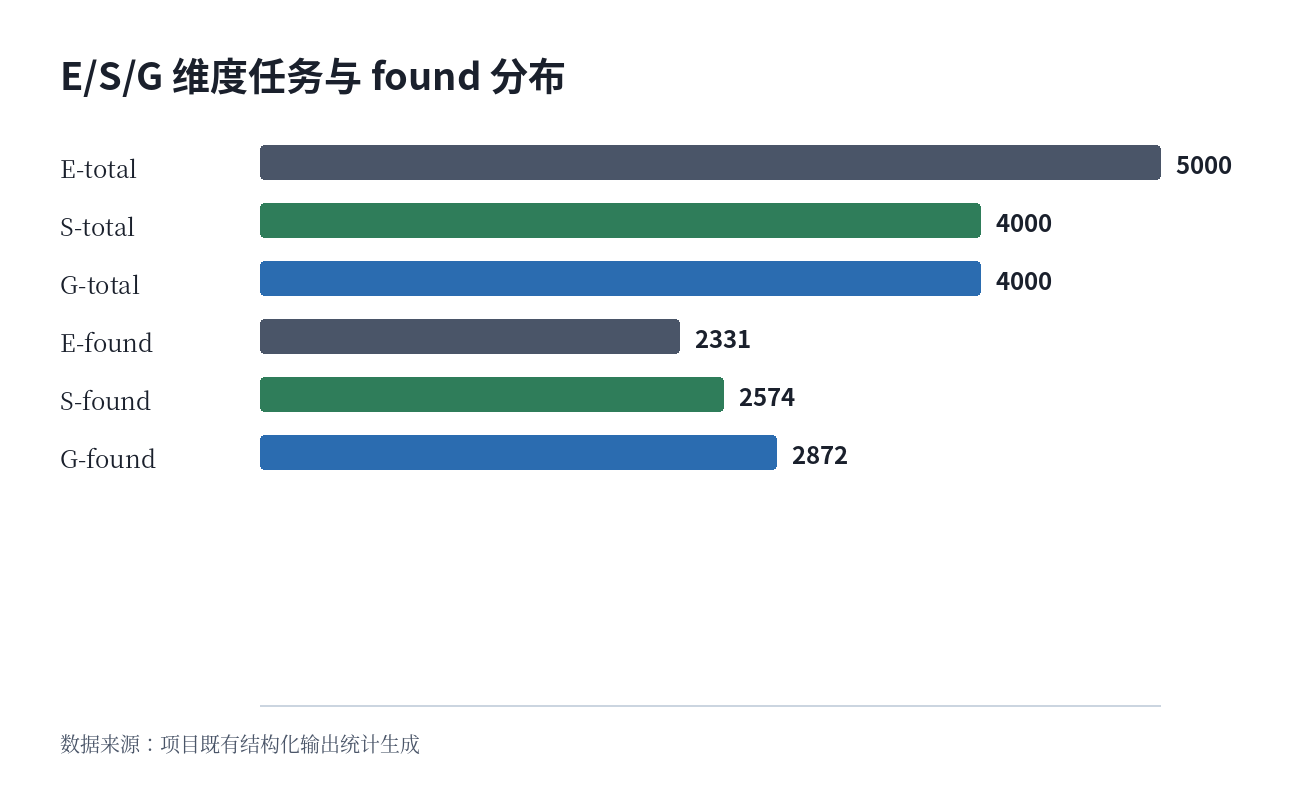
\includegraphics[width=0.9\linewidth]{fig_dimension_result.png}
\caption{E/S/G 维度任务与 found 分布}
\label{fig:dimension-result}
\end{figure}

\subsection{指标类型结果分析}
按类型看，定量任务 7000 条，found 3217 条；机制性布尔任务 3000 条，found 2244 条；定性任务 3000 条，found 2316 条。定量指标 found 比例相对较低，原因在于其同时要求指标名、数值和单位三类证据闭合：表格表头缺失、单位位于上一行、同一表格含多年度数值、百分比与人数混排，都会使模型难以在证据范围内给出稳定输出。定性指标和机制性布尔指标的证据通常是段落文本，候选召回更容易命中；但二者的风险不同。定性指标的主要问题是证据片段可能过短，不能完整支撑结论；机制性布尔指标的主要问题是标题、目录或章节名含有“治理架构”“反腐败”等词，但正文未给出制度或措施内容，此时若直接判定 true，就会形成标题式机制误判。因此，本文在 schema 约束中要求布尔 found 必须给出机制、制度或行动证据，并在质量诊断中单独设置标题式机制风险。

\begin{figure}[htbp]
\centering
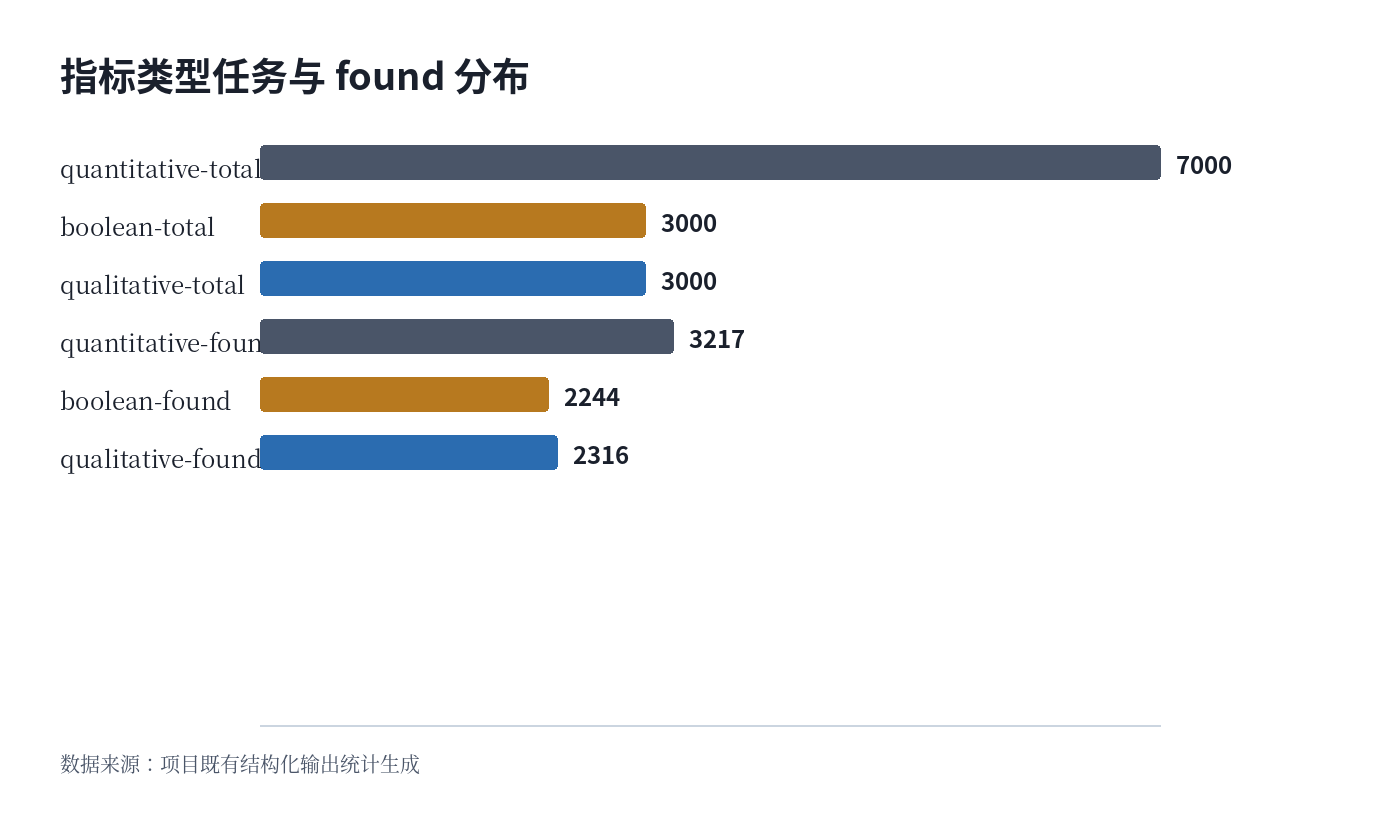
\includegraphics[width=0.92\linewidth]{fig_type_result.png}
\caption{指标类型任务与 found 分布}
\label{fig:type-result}
\end{figure}

\subsection{定量字段与运行耗时}
质量指标显示，定量 found 中 value 缺失 0 条，unit 缺失 3 条，定量字段不完整 3 条；证据为空 0 条，证据过短 27 条；后处理修复 109 条。这说明字段约束对定量输出有明显筛选作用：当证据无法同时支撑数值和单位时，多数样本被保守地留在 missing 或风险样本中，而不是生成不可核验数值。耗时记录显示，逐任务记录字段求和为 9064.17 秒，平均 0.70 秒；正式批处理墙钟耗时为 4930.803 秒。两种口径分别反映任务级记录和批处理总运行时间，不能直接相互替代。

\subsection{风险样本分析}
质量诊断共识别 164 个具体风险样本，其中 high 36 个、medium 72 个、low 56 个。按风险类型看，零事件归一 56 个、证据过短 39 个、标题式机制证据 33 个、比例误作数量 32 个、value/unit 缺失 3 个、金额误作数量 1 个。这些样本不是最终错误集，而是用于复核排序的风险集合。零事件风险集中出现，是因为 ESG 报告常用“未发生重大安全事故”“无工亡”等自然语言表达，系统需要将其归一为 0，但仍需确认事件边界。比例误作数量风险主要来自“女性董事占比”“独立董事比例”等语境，这些百分比不应被抽成董事人数或事故次数。标题式机制风险则反映 boolean 指标的典型难点：标题能说明报告有相关章节，但不能单独证明企业建立了制度或执行了措施。

\begin{figure}[htbp]
\centering
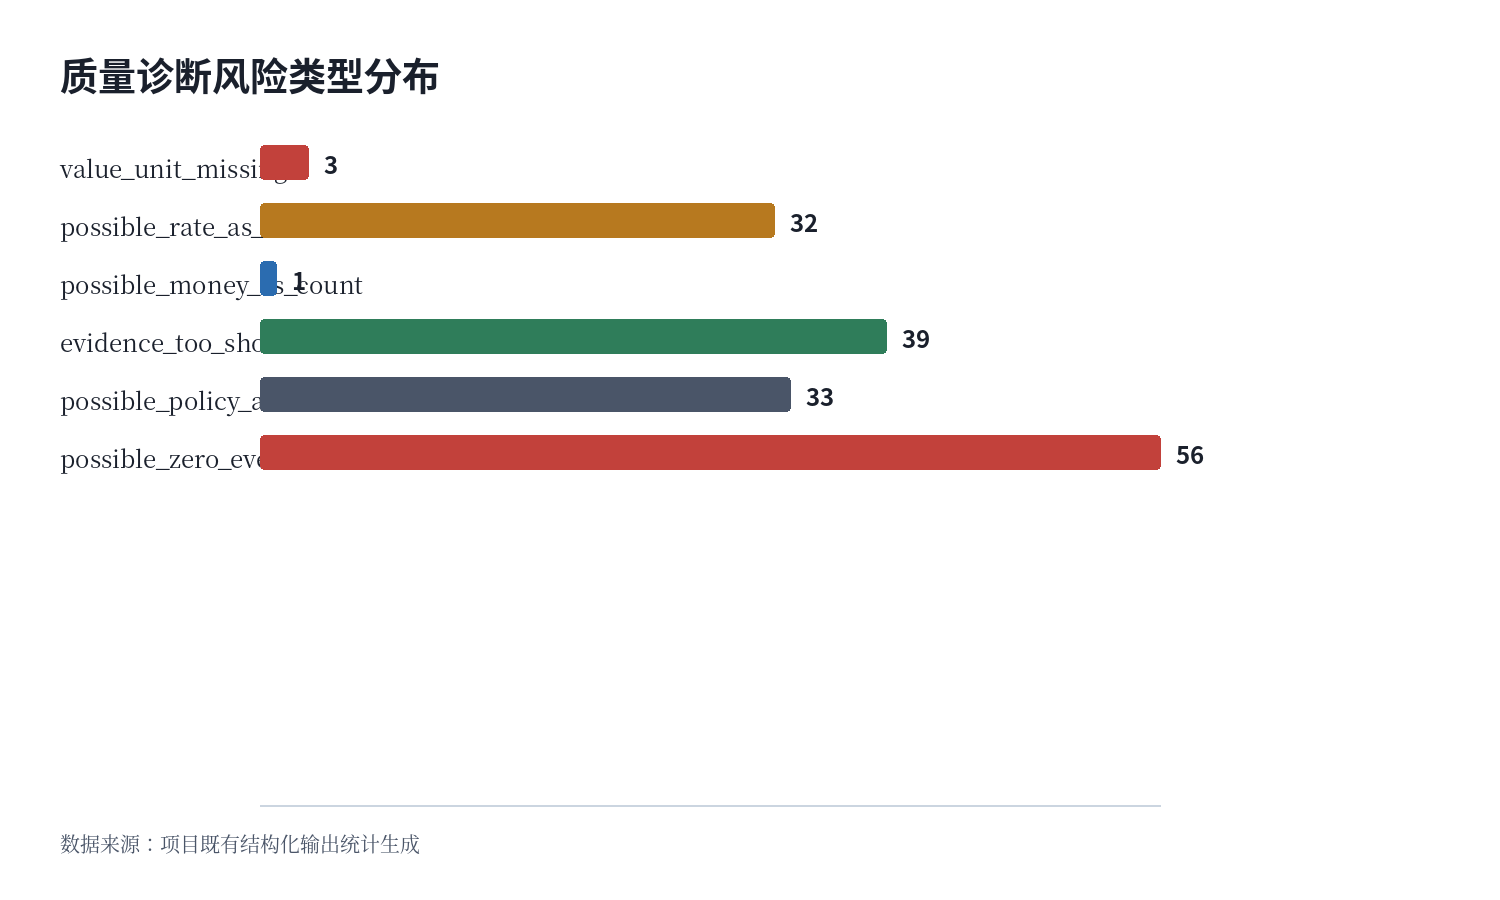
\includegraphics[width=0.95\linewidth]{fig_risk_distribution.png}
\caption{质量诊断风险类型分布}
\label{fig:risk-distribution}
\end{figure}

\begin{figure}[htbp]
\centering
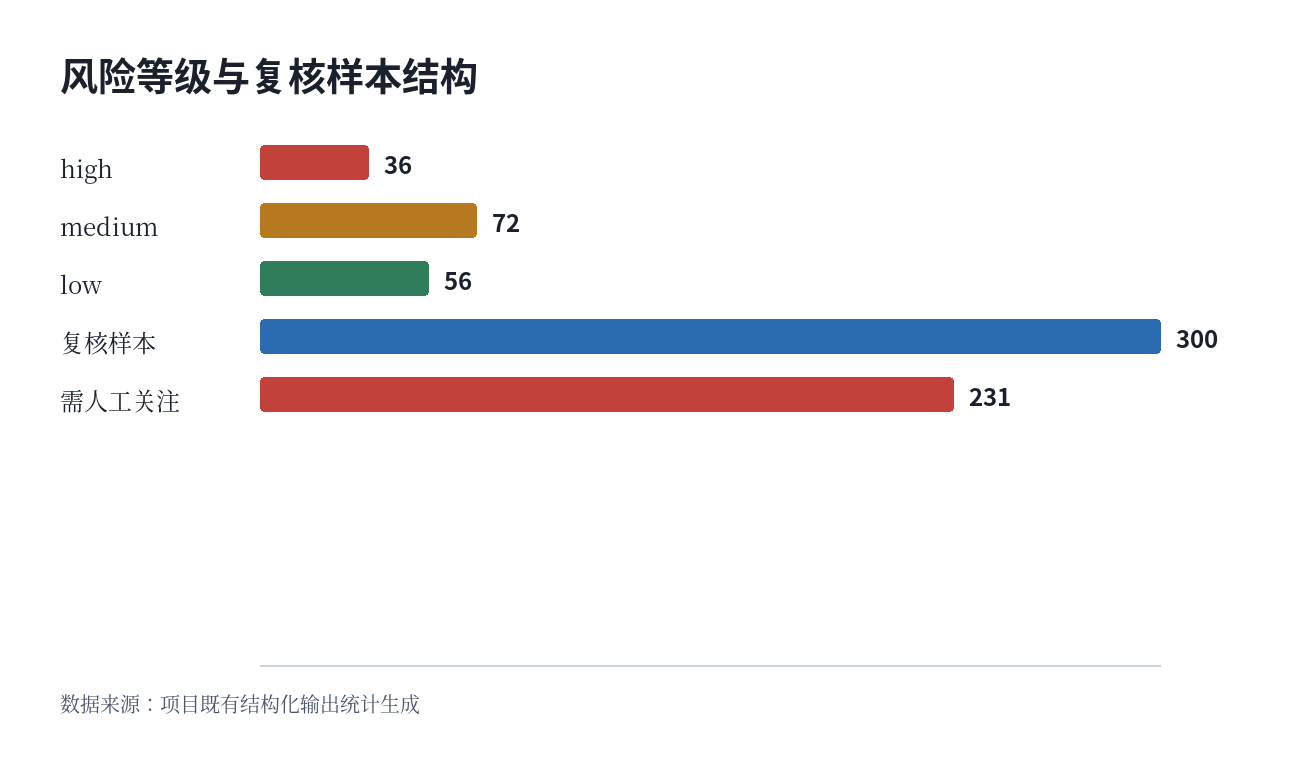
\includegraphics[width=0.9\linewidth]{fig_risk_level.png}
\caption{风险等级与复核样本结构}
\label{fig:risk-level}
\end{figure}

\subsection{典型抽取案例}
\begingroup
\small
\setlength{\tabcolsep}{3pt}
\renewcommand{\arraystretch}{1.18}
\begin{longtable}{@{}p{2.0cm}p{2.0cm}p{2.3cm}p{4.9cm}p{2.55cm}@{}}
\caption{典型抽取与风险样本}\label{tab:typical-cases}\\
\toprule
案例类型 & 指标 & 抽取输出 & 原文证据摘录 & 复核说明 \\
\midrule
\endfirsthead
\toprule
案例类型 & 指标 & 抽取输出 & 原文证据摘录 & 复核说明 \\
\midrule
\endhead
定量抽取 & 温室气体排放总量 & 117,319.54 吨二氧化碳当量 & 温室气体排放总量 | 吨二氧化碳当量 | 117,319.54 | 113,126.46 & 表格证据同时给出指标名、数值和单位。 \\
定性抽取 & 绿色产品与服务 & 多款核心产品通过绿色产品认证，推动绿色产品认证工作，将绿 & 多款核心产品通过绿色产品认证，推动绿色产品认证工作，将绿色低碳理念融入产品的设计开发、生产制造、回收利用等环... & 原文片段能够支撑定性描述。 \\
机制判定 & 碳排放管理措施 & true & 康佳高度重视气候变化带来的机遇与挑战，扎实推进碳排放管理工作，以EHSQ管理体系为支撑，成立EHSQ委员会，... & 证据包含机制、组织或措施，不只是标题。 \\
单位缺失风险 & 董事会多元化 & 7:2 & 董事会成员男女比例为 7 : 2 & 输出缺少单位或单位语境不完整，需核对表头。 \\
单位缺失风险 & 独立董事占比 & 6:3 & 非独立董事和独立董事比例为 6 : 3 & 输出缺少单位或单位语境不完整，需核对表头。 \\
单位缺失风险 & 独立董事占比 & 2 & 独立董事2位 非独立董事1位 独董担任主任委员 & 输出缺少单位或单位语境不完整，需核对表头。 \\
比例误作数量风险 & 董事会人数 & 9 人 & 公司董事会由9名董事构成。其中，非独立董事6名，独立董事3名；女性董事3名，占比33\%。 & 证据含比例表达，需确认是否误作数量。 \\
比例误作数量风险 & 客户投诉 & 100\% & 客户投诉处理率 | 100\% & 证据含比例表达，需确认是否误作数量。 \\
\bottomrule
\end{longtable}

\endgroup

定量样例中，温室气体排放总量可从表格证据中抽取 value 与 unit；定性样例中，绿色产品与服务需要保留语义完整的原文片段；机制性布尔样例中，碳排放管理措施必须有制度或组织安排证据。风险样例则展示了单位缺失、比例语境、金额单位、零事件和过短证据等复核重点。通过将这些样例放入系统页面，评审者可直接按 report\_id、indicator\_id 和 block\_id 回到具体证据。

\subsection{系统展示与复核流程}
系统总览页展示报告数、指标数、任务数、found/missing/error 运行状态、后处理修复数和风险样本数，真实页面见 \figref{fig:system-ui-overview}。公司视角可查看单份报告的所有指标结果，指标视角可横向查看某一指标在 200 份报告中的披露与字段样例，分别见 \figref{fig:system-ui-company} 与 \figref{fig:system-ui-indicator}。证据核验页支持按维度、指标类型、状态、风险标签、报告和指标名称筛选，筛选结果表直接展示 evidence\_quote、page\_no 和 block\_id，见 \figref{fig:system-ui-evidence}。高风险样本页按 risk\_level 与 suspected\_issue\_type 组织复核，见 \figref{fig:system-ui-risk}。新报告接入页展示单份 PDF 的处理入口和预期输出文件。该系统把结构化字段与证据字段放在同一界面中，避免结果展示脱离证据来源。

\newpage
\section{模型评价}
\subsection{模型优点}
本文方法的主要优点在于：一是将 PDF 解析为内容块，保留页码和块号，使结构化结果可以回溯；二是用 ESG-65 指标体系区分定量、定性和机制性指标，避免所有指标共用单一抽取模板；三是通过候选证据召回降低长文档噪声，使 qwen3 在局部证据内完成语义抽取；四是使用固定 JSON schema、后处理和质量诊断提高字段稳定性；五是通过 Streamlit 系统把结果查看、证据定位、风险样本和下载功能串联起来。

\subsection{局限性}
本文仍存在客观局限。关键词召回对同义表达和行业特定术语仍可能漏召；跨页表格、图片化文字和复杂合并单元格可能在解析阶段损失上下文；部分 ESG 指标的行业口径差异较大，同一字段在不同行业中的含义可能不同；自动质量诊断不能替代完整人工标注；当前模型不构建 ESG 评分模型，也不输出企业优劣排序；大语言模型输出仍需要 evidence\_quote 与风险规则共同约束。

\subsection{改进方向}
后续可从六个方向改进：引入 embedding 召回以补充关键词漏召；增强跨页表格结构恢复；建立行业口径规则和单位标准化字典；构建覆盖多行业的人工真值集；对高风险指标设计专项规则；进一步优化系统界面的证据跳转、批注和复核记录功能。

\section{结论}
本文围绕 ESG 长 PDF 报告中的定量与定性指标识别，建立了证据约束型结构化抽取模型。模型以 200 份报告和 ESG-65 指标体系为输入，将任务拆解为 13000 个 report-indicator 结构化抽取问题，通过 MinerU 解析、内容块建模、候选证据召回、qwen3 约束抽取、后处理和质量诊断生成可追溯结果。实验结果显示，正式批次形成 7777 条 found 与 5223 条 missing 运行结果，并保留完整 page\_no 与 block\_id 字段；质量诊断进一步识别 164 个具体风险样本，为人工复核提供优先级。最后，Streamlit 系统将公司视角、指标视角、证据核验、风险样本和新报告接入整合为闭环，使结构化结果不仅可输出为 CSV/JSON，也可被逐条核验。

\newpage
\section{参考文献}
\printbibliography[heading=none]

\newpage
\appendix
\section{关键模型代码}
\subsection{内容块构造与候选召回}
\begin{Verbatim}[fontsize=\small,frame=single]
for report in reports:
    blocks = parse_pdf_to_blocks(report)
    for indicator in indicators:
        candidates = []
        for block in blocks:
            score = keyword_score(block, indicator)
            score += unit_score(block, indicator)
            score += block_type_score(block)
            score += position_score(block)
            if score > 0:
                candidates.append((score, block))
        evidence = top_k(candidates, k)
        if evidence is empty:
            emit_missing(report, indicator)
        else:
            constrained_extract(report, indicator, evidence)
\end{Verbatim}

\subsection{证据约束抽取与后处理}
\begin{Verbatim}[fontsize=\small,frame=single]
def constrained_extract(report, indicator, evidence):
    prompt = build_prompt(indicator, evidence)
    raw = call_llm(prompt)
    record = parse_json_schema(raw)

    if record.status == "found":
        require_quote_from_evidence(record.evidence_quote, evidence)
        require_trace_fields(record.page_no, record.block_id)
        if indicator.type == "quantitative":
            require_value_and_unit(
                record.value, record.unit
            )
        if indicator.type == "boolean":
            reject_title_only_evidence(
                record.evidence_quote
            )

    record = normalize_zero_event(record)
    record = repair_common_unit(record)
    record.risk_tag = diagnose_risk(record, indicator, evidence)
    return record
\end{Verbatim}




\end{document}
